\documentclass[10pt, a4paper]{article}

    \usepackage[breakable]{tcolorbox}
    \usepackage{parskip} % Stop auto-indenting (to mimic markdown behaviour)
    
    \usepackage{iftex}
    \ifPDFTeX
    	\usepackage[T1]{fontenc}
    	\usepackage{mathpazo}
    \else
    	\usepackage{fontspec}
    \fi

    % Basic figure setup, for now with no caption control since it's done
    % automatically by Pandoc (which extracts ![](path) syntax from Markdown).
    \usepackage{graphicx}
    % Maintain compatibility with old templates. Remove in nbconvert 6.0
    \let\Oldincludegraphics\includegraphics

    \usepackage[Export]{adjustbox} % Used to constrain images to a maximum size
    \adjustboxset{max size={0.9\linewidth}{0.9\paperheight}}
    \usepackage{float}
    \floatplacement{figure}{H} % forces figures to be placed at the correct location
    \usepackage{xcolor} % Allow colors to be defined
    \usepackage{enumerate} % Needed for markdown enumerations to work
    \usepackage{geometry} % Used to adjust the document margins
    \usepackage{amsmath} % Equations
    \usepackage{amssymb} % Equations
    \usepackage{textcomp} % defines textquotesingle
    % Hack from http://tex.stackexchange.com/a/47451/13684:
    \AtBeginDocument{%
        \def\PYZsq{\textquotesingle}% Upright quotes in Pygmentized code
    }
    \usepackage{upquote} % Upright quotes for verbatim code
    \usepackage{eurosym} % defines \euro
    \usepackage[mathletters]{ucs} % Extended unicode (utf-8) support
    \usepackage{fancyvrb} % verbatim replacement that allows latex
    \usepackage{grffile} % extends the file name processing of package graphics 
                         % to support a larger range
    \makeatletter % fix for grffile with XeLaTeX
    \def\Gread@@xetex#1{%
      \IfFileExists{"\Gin@base".bb}%
      {\Gread@eps{\Gin@base.bb}}%
      {\Gread@@xetex@aux#1}%
    }
    \makeatother

    % The hyperref package gives us a pdf with properly built
    % internal navigation ('pdf bookmarks' for the table of contents,
    % internal cross-reference links, web links for URLs, etc.)
    \usepackage{hyperref}
    % The default LaTeX title has an obnoxious amount of whitespace. By default,
    % titling removes some of it. It also provides customization options.
    \usepackage{titling}
    \usepackage{longtable} % longtable support required by pandoc >1.10
    \usepackage{booktabs}  % table support for pandoc > 1.12.2
    \usepackage[inline]{enumitem} % IRkernel/repr support (it uses the enumerate* environment)
    \usepackage[normalem]{ulem} % ulem is needed to support strikethroughs (\sout)
                                % normalem makes italics be italics, not underlines
    \usepackage{mathrsfs}
    

    
    % Colors for the hyperref package
    \definecolor{urlcolor}{rgb}{0,.145,.698}
    \definecolor{linkcolor}{rgb}{.71,0.21,0.01}
    \definecolor{citecolor}{rgb}{.12,.54,.11}

    % ANSI colors
    \definecolor{ansi-black}{HTML}{3E424D}
    \definecolor{ansi-black-intense}{HTML}{282C36}
    \definecolor{ansi-red}{HTML}{E75C58}
    \definecolor{ansi-red-intense}{HTML}{B22B31}
    \definecolor{ansi-green}{HTML}{00A250}
    \definecolor{ansi-green-intense}{HTML}{007427}
    \definecolor{ansi-yellow}{HTML}{DDB62B}
    \definecolor{ansi-yellow-intense}{HTML}{B27D12}
    \definecolor{ansi-blue}{HTML}{208FFB}
    \definecolor{ansi-blue-intense}{HTML}{0065CA}
    \definecolor{ansi-magenta}{HTML}{D160C4}
    \definecolor{ansi-magenta-intense}{HTML}{A03196}
    \definecolor{ansi-cyan}{HTML}{60C6C8}
    \definecolor{ansi-cyan-intense}{HTML}{258F8F}
    \definecolor{ansi-white}{HTML}{C5C1B4}
    \definecolor{ansi-white-intense}{HTML}{A1A6B2}
    \definecolor{ansi-default-inverse-fg}{HTML}{FFFFFF}
    \definecolor{ansi-default-inverse-bg}{HTML}{000000}

    % commands and environments needed by pandoc snippets
    % extracted from the output of `pandoc -s`
    \providecommand{\tightlist}{%
      \setlength{\itemsep}{0pt}\setlength{\parskip}{0pt}}
    \DefineVerbatimEnvironment{Highlighting}{Verbatim}{commandchars=\\\{\}}
    % Add ',fontsize=\small' for more characters per line
    \newenvironment{Shaded}{}{}
    \newcommand{\KeywordTok}[1]{\textcolor[rgb]{0.00,0.44,0.13}{\textbf{{#1}}}}
    \newcommand{\DataTypeTok}[1]{\textcolor[rgb]{0.56,0.13,0.00}{{#1}}}
    \newcommand{\DecValTok}[1]{\textcolor[rgb]{0.25,0.63,0.44}{{#1}}}
    \newcommand{\BaseNTok}[1]{\textcolor[rgb]{0.25,0.63,0.44}{{#1}}}
    \newcommand{\FloatTok}[1]{\textcolor[rgb]{0.25,0.63,0.44}{{#1}}}
    \newcommand{\CharTok}[1]{\textcolor[rgb]{0.25,0.44,0.63}{{#1}}}
    \newcommand{\StringTok}[1]{\textcolor[rgb]{0.25,0.44,0.63}{{#1}}}
    \newcommand{\CommentTok}[1]{\textcolor[rgb]{0.38,0.63,0.69}{\textit{{#1}}}}
    \newcommand{\OtherTok}[1]{\textcolor[rgb]{0.00,0.44,0.13}{{#1}}}
    \newcommand{\AlertTok}[1]{\textcolor[rgb]{1.00,0.00,0.00}{\textbf{{#1}}}}
    \newcommand{\FunctionTok}[1]{\textcolor[rgb]{0.02,0.16,0.49}{{#1}}}
    \newcommand{\RegionMarkerTok}[1]{{#1}}
    \newcommand{\ErrorTok}[1]{\textcolor[rgb]{1.00,0.00,0.00}{\textbf{{#1}}}}
    \newcommand{\NormalTok}[1]{{#1}}
    
    % Additional commands for more recent versions of Pandoc
    \newcommand{\ConstantTok}[1]{\textcolor[rgb]{0.53,0.00,0.00}{{#1}}}
    \newcommand{\SpecialCharTok}[1]{\textcolor[rgb]{0.25,0.44,0.63}{{#1}}}
    \newcommand{\VerbatimStringTok}[1]{\textcolor[rgb]{0.25,0.44,0.63}{{#1}}}
    \newcommand{\SpecialStringTok}[1]{\textcolor[rgb]{0.73,0.40,0.53}{{#1}}}
    \newcommand{\ImportTok}[1]{{#1}}
    \newcommand{\DocumentationTok}[1]{\textcolor[rgb]{0.73,0.13,0.13}{\textit{{#1}}}}
    \newcommand{\AnnotationTok}[1]{\textcolor[rgb]{0.38,0.63,0.69}{\textbf{\textit{{#1}}}}}
    \newcommand{\CommentVarTok}[1]{\textcolor[rgb]{0.38,0.63,0.69}{\textbf{\textit{{#1}}}}}
    \newcommand{\VariableTok}[1]{\textcolor[rgb]{0.10,0.09,0.49}{{#1}}}
    \newcommand{\ControlFlowTok}[1]{\textcolor[rgb]{0.00,0.44,0.13}{\textbf{{#1}}}}
    \newcommand{\OperatorTok}[1]{\textcolor[rgb]{0.40,0.40,0.40}{{#1}}}
    \newcommand{\BuiltInTok}[1]{{#1}}
    \newcommand{\ExtensionTok}[1]{{#1}}
    \newcommand{\PreprocessorTok}[1]{\textcolor[rgb]{0.74,0.48,0.00}{{#1}}}
    \newcommand{\AttributeTok}[1]{\textcolor[rgb]{0.49,0.56,0.16}{{#1}}}
    \newcommand{\InformationTok}[1]{\textcolor[rgb]{0.38,0.63,0.69}{\textbf{\textit{{#1}}}}}
    \newcommand{\WarningTok}[1]{\textcolor[rgb]{0.38,0.63,0.69}{\textbf{\textit{{#1}}}}}
    
    
    % Define a nice break command that doesn't care if a line doesn't already
    % exist.
    \def\br{\hspace*{\fill} \\* }
    % Math Jax compatibility definitions
    \def\gt{>}
    \def\lt{<}
    \let\Oldtex\TeX
    \let\Oldlatex\LaTeX
    \renewcommand{\TeX}{\textrm{\Oldtex}}
    \renewcommand{\LaTeX}{\textrm{\Oldlatex}}
    % Document parameters
    % Document title

    
% Pygments definitions
\makeatletter
\def\PY@reset{\let\PY@it=\relax \let\PY@bf=\relax%
    \let\PY@ul=\relax \let\PY@tc=\relax%
    \let\PY@bc=\relax \let\PY@ff=\relax}
\def\PY@tok#1{\csname PY@tok@#1\endcsname}
\def\PY@toks#1+{\ifx\relax#1\empty\else%
    \PY@tok{#1}\expandafter\PY@toks\fi}
\def\PY@do#1{\PY@bc{\PY@tc{\PY@ul{%
    \PY@it{\PY@bf{\PY@ff{#1}}}}}}}
\def\PY#1#2{\PY@reset\PY@toks#1+\relax+\PY@do{#2}}

\expandafter\def\csname PY@tok@w\endcsname{\def\PY@tc##1{\textcolor[rgb]{0.73,0.73,0.73}{##1}}}
\expandafter\def\csname PY@tok@c\endcsname{\let\PY@it=\textit\def\PY@tc##1{\textcolor[rgb]{0.25,0.50,0.50}{##1}}}
\expandafter\def\csname PY@tok@cp\endcsname{\def\PY@tc##1{\textcolor[rgb]{0.74,0.48,0.00}{##1}}}
\expandafter\def\csname PY@tok@k\endcsname{\let\PY@bf=\textbf\def\PY@tc##1{\textcolor[rgb]{0.00,0.50,0.00}{##1}}}
\expandafter\def\csname PY@tok@kp\endcsname{\def\PY@tc##1{\textcolor[rgb]{0.00,0.50,0.00}{##1}}}
\expandafter\def\csname PY@tok@kt\endcsname{\def\PY@tc##1{\textcolor[rgb]{0.69,0.00,0.25}{##1}}}
\expandafter\def\csname PY@tok@o\endcsname{\def\PY@tc##1{\textcolor[rgb]{0.40,0.40,0.40}{##1}}}
\expandafter\def\csname PY@tok@ow\endcsname{\let\PY@bf=\textbf\def\PY@tc##1{\textcolor[rgb]{0.67,0.13,1.00}{##1}}}
\expandafter\def\csname PY@tok@nb\endcsname{\def\PY@tc##1{\textcolor[rgb]{0.00,0.50,0.00}{##1}}}
\expandafter\def\csname PY@tok@nf\endcsname{\def\PY@tc##1{\textcolor[rgb]{0.00,0.00,1.00}{##1}}}
\expandafter\def\csname PY@tok@nc\endcsname{\let\PY@bf=\textbf\def\PY@tc##1{\textcolor[rgb]{0.00,0.00,1.00}{##1}}}
\expandafter\def\csname PY@tok@nn\endcsname{\let\PY@bf=\textbf\def\PY@tc##1{\textcolor[rgb]{0.00,0.00,1.00}{##1}}}
\expandafter\def\csname PY@tok@ne\endcsname{\let\PY@bf=\textbf\def\PY@tc##1{\textcolor[rgb]{0.82,0.25,0.23}{##1}}}
\expandafter\def\csname PY@tok@nv\endcsname{\def\PY@tc##1{\textcolor[rgb]{0.10,0.09,0.49}{##1}}}
\expandafter\def\csname PY@tok@no\endcsname{\def\PY@tc##1{\textcolor[rgb]{0.53,0.00,0.00}{##1}}}
\expandafter\def\csname PY@tok@nl\endcsname{\def\PY@tc##1{\textcolor[rgb]{0.63,0.63,0.00}{##1}}}
\expandafter\def\csname PY@tok@ni\endcsname{\let\PY@bf=\textbf\def\PY@tc##1{\textcolor[rgb]{0.60,0.60,0.60}{##1}}}
\expandafter\def\csname PY@tok@na\endcsname{\def\PY@tc##1{\textcolor[rgb]{0.49,0.56,0.16}{##1}}}
\expandafter\def\csname PY@tok@nt\endcsname{\let\PY@bf=\textbf\def\PY@tc##1{\textcolor[rgb]{0.00,0.50,0.00}{##1}}}
\expandafter\def\csname PY@tok@nd\endcsname{\def\PY@tc##1{\textcolor[rgb]{0.67,0.13,1.00}{##1}}}
\expandafter\def\csname PY@tok@s\endcsname{\def\PY@tc##1{\textcolor[rgb]{0.73,0.13,0.13}{##1}}}
\expandafter\def\csname PY@tok@sd\endcsname{\let\PY@it=\textit\def\PY@tc##1{\textcolor[rgb]{0.73,0.13,0.13}{##1}}}
\expandafter\def\csname PY@tok@si\endcsname{\let\PY@bf=\textbf\def\PY@tc##1{\textcolor[rgb]{0.73,0.40,0.53}{##1}}}
\expandafter\def\csname PY@tok@se\endcsname{\let\PY@bf=\textbf\def\PY@tc##1{\textcolor[rgb]{0.73,0.40,0.13}{##1}}}
\expandafter\def\csname PY@tok@sr\endcsname{\def\PY@tc##1{\textcolor[rgb]{0.73,0.40,0.53}{##1}}}
\expandafter\def\csname PY@tok@ss\endcsname{\def\PY@tc##1{\textcolor[rgb]{0.10,0.09,0.49}{##1}}}
\expandafter\def\csname PY@tok@sx\endcsname{\def\PY@tc##1{\textcolor[rgb]{0.00,0.50,0.00}{##1}}}
\expandafter\def\csname PY@tok@m\endcsname{\def\PY@tc##1{\textcolor[rgb]{0.40,0.40,0.40}{##1}}}
\expandafter\def\csname PY@tok@gh\endcsname{\let\PY@bf=\textbf\def\PY@tc##1{\textcolor[rgb]{0.00,0.00,0.50}{##1}}}
\expandafter\def\csname PY@tok@gu\endcsname{\let\PY@bf=\textbf\def\PY@tc##1{\textcolor[rgb]{0.50,0.00,0.50}{##1}}}
\expandafter\def\csname PY@tok@gd\endcsname{\def\PY@tc##1{\textcolor[rgb]{0.63,0.00,0.00}{##1}}}
\expandafter\def\csname PY@tok@gi\endcsname{\def\PY@tc##1{\textcolor[rgb]{0.00,0.63,0.00}{##1}}}
\expandafter\def\csname PY@tok@gr\endcsname{\def\PY@tc##1{\textcolor[rgb]{1.00,0.00,0.00}{##1}}}
\expandafter\def\csname PY@tok@ge\endcsname{\let\PY@it=\textit}
\expandafter\def\csname PY@tok@gs\endcsname{\let\PY@bf=\textbf}
\expandafter\def\csname PY@tok@gp\endcsname{\let\PY@bf=\textbf\def\PY@tc##1{\textcolor[rgb]{0.00,0.00,0.50}{##1}}}
\expandafter\def\csname PY@tok@go\endcsname{\def\PY@tc##1{\textcolor[rgb]{0.53,0.53,0.53}{##1}}}
\expandafter\def\csname PY@tok@gt\endcsname{\def\PY@tc##1{\textcolor[rgb]{0.00,0.27,0.87}{##1}}}
\expandafter\def\csname PY@tok@err\endcsname{\def\PY@bc##1{\setlength{\fboxsep}{0pt}\fcolorbox[rgb]{1.00,0.00,0.00}{1,1,1}{\strut ##1}}}
\expandafter\def\csname PY@tok@kc\endcsname{\let\PY@bf=\textbf\def\PY@tc##1{\textcolor[rgb]{0.00,0.50,0.00}{##1}}}
\expandafter\def\csname PY@tok@kd\endcsname{\let\PY@bf=\textbf\def\PY@tc##1{\textcolor[rgb]{0.00,0.50,0.00}{##1}}}
\expandafter\def\csname PY@tok@kn\endcsname{\let\PY@bf=\textbf\def\PY@tc##1{\textcolor[rgb]{0.00,0.50,0.00}{##1}}}
\expandafter\def\csname PY@tok@kr\endcsname{\let\PY@bf=\textbf\def\PY@tc##1{\textcolor[rgb]{0.00,0.50,0.00}{##1}}}
\expandafter\def\csname PY@tok@bp\endcsname{\def\PY@tc##1{\textcolor[rgb]{0.00,0.50,0.00}{##1}}}
\expandafter\def\csname PY@tok@fm\endcsname{\def\PY@tc##1{\textcolor[rgb]{0.00,0.00,1.00}{##1}}}
\expandafter\def\csname PY@tok@vc\endcsname{\def\PY@tc##1{\textcolor[rgb]{0.10,0.09,0.49}{##1}}}
\expandafter\def\csname PY@tok@vg\endcsname{\def\PY@tc##1{\textcolor[rgb]{0.10,0.09,0.49}{##1}}}
\expandafter\def\csname PY@tok@vi\endcsname{\def\PY@tc##1{\textcolor[rgb]{0.10,0.09,0.49}{##1}}}
\expandafter\def\csname PY@tok@vm\endcsname{\def\PY@tc##1{\textcolor[rgb]{0.10,0.09,0.49}{##1}}}
\expandafter\def\csname PY@tok@sa\endcsname{\def\PY@tc##1{\textcolor[rgb]{0.73,0.13,0.13}{##1}}}
\expandafter\def\csname PY@tok@sb\endcsname{\def\PY@tc##1{\textcolor[rgb]{0.73,0.13,0.13}{##1}}}
\expandafter\def\csname PY@tok@sc\endcsname{\def\PY@tc##1{\textcolor[rgb]{0.73,0.13,0.13}{##1}}}
\expandafter\def\csname PY@tok@dl\endcsname{\def\PY@tc##1{\textcolor[rgb]{0.73,0.13,0.13}{##1}}}
\expandafter\def\csname PY@tok@s2\endcsname{\def\PY@tc##1{\textcolor[rgb]{0.73,0.13,0.13}{##1}}}
\expandafter\def\csname PY@tok@sh\endcsname{\def\PY@tc##1{\textcolor[rgb]{0.73,0.13,0.13}{##1}}}
\expandafter\def\csname PY@tok@s1\endcsname{\def\PY@tc##1{\textcolor[rgb]{0.73,0.13,0.13}{##1}}}
\expandafter\def\csname PY@tok@mb\endcsname{\def\PY@tc##1{\textcolor[rgb]{0.40,0.40,0.40}{##1}}}
\expandafter\def\csname PY@tok@mf\endcsname{\def\PY@tc##1{\textcolor[rgb]{0.40,0.40,0.40}{##1}}}
\expandafter\def\csname PY@tok@mh\endcsname{\def\PY@tc##1{\textcolor[rgb]{0.40,0.40,0.40}{##1}}}
\expandafter\def\csname PY@tok@mi\endcsname{\def\PY@tc##1{\textcolor[rgb]{0.40,0.40,0.40}{##1}}}
\expandafter\def\csname PY@tok@il\endcsname{\def\PY@tc##1{\textcolor[rgb]{0.40,0.40,0.40}{##1}}}
\expandafter\def\csname PY@tok@mo\endcsname{\def\PY@tc##1{\textcolor[rgb]{0.40,0.40,0.40}{##1}}}
\expandafter\def\csname PY@tok@ch\endcsname{\let\PY@it=\textit\def\PY@tc##1{\textcolor[rgb]{0.25,0.50,0.50}{##1}}}
\expandafter\def\csname PY@tok@cm\endcsname{\let\PY@it=\textit\def\PY@tc##1{\textcolor[rgb]{0.25,0.50,0.50}{##1}}}
\expandafter\def\csname PY@tok@cpf\endcsname{\let\PY@it=\textit\def\PY@tc##1{\textcolor[rgb]{0.25,0.50,0.50}{##1}}}
\expandafter\def\csname PY@tok@c1\endcsname{\let\PY@it=\textit\def\PY@tc##1{\textcolor[rgb]{0.25,0.50,0.50}{##1}}}
\expandafter\def\csname PY@tok@cs\endcsname{\let\PY@it=\textit\def\PY@tc##1{\textcolor[rgb]{0.25,0.50,0.50}{##1}}}

\def\PYZbs{\char`\\}
\def\PYZus{\char`\_}
\def\PYZob{\char`\{}
\def\PYZcb{\char`\}}
\def\PYZca{\char`\^}
\def\PYZam{\char`\&}
\def\PYZlt{\char`\<}
\def\PYZgt{\char`\>}
\def\PYZsh{\char`\#}
\def\PYZpc{\char`\%}
\def\PYZdl{\char`\$}
\def\PYZhy{\char`\-}
\def\PYZsq{\char`\'}
\def\PYZdq{\char`\"}
\def\PYZti{\char`\~}
% for compatibility with earlier versions
\def\PYZat{@}
\def\PYZlb{[}
\def\PYZrb{]}
\makeatother


    % For linebreaks inside Verbatim environment from package fancyvrb. 
    \makeatletter
        \newbox\Wrappedcontinuationbox 
        \newbox\Wrappedvisiblespacebox 
        \newcommand*\Wrappedvisiblespace {\textcolor{red}{\textvisiblespace}} 
        \newcommand*\Wrappedcontinuationsymbol {\textcolor{red}{\llap{\tiny$\m@th\hookrightarrow$}}} 
        \newcommand*\Wrappedcontinuationindent {3ex } 
        \newcommand*\Wrappedafterbreak {\kern\Wrappedcontinuationindent\copy\Wrappedcontinuationbox} 
        % Take advantage of the already applied Pygments mark-up to insert 
        % potential linebreaks for TeX processing. 
        %        {, <, #, %, $, ' and ": go to next line. 
        %        _, }, ^, &, >, - and ~: stay at end of broken line. 
        % Use of \textquotesingle for straight quote. 
        \newcommand*\Wrappedbreaksatspecials {% 
            \def\PYGZus{\discretionary{\char`\_}{\Wrappedafterbreak}{\char`\_}}% 
            \def\PYGZob{\discretionary{}{\Wrappedafterbreak\char`\{}{\char`\{}}% 
            \def\PYGZcb{\discretionary{\char`\}}{\Wrappedafterbreak}{\char`\}}}% 
            \def\PYGZca{\discretionary{\char`\^}{\Wrappedafterbreak}{\char`\^}}% 
            \def\PYGZam{\discretionary{\char`\&}{\Wrappedafterbreak}{\char`\&}}% 
            \def\PYGZlt{\discretionary{}{\Wrappedafterbreak\char`\<}{\char`\<}}% 
            \def\PYGZgt{\discretionary{\char`\>}{\Wrappedafterbreak}{\char`\>}}% 
            \def\PYGZsh{\discretionary{}{\Wrappedafterbreak\char`\#}{\char`\#}}% 
            \def\PYGZpc{\discretionary{}{\Wrappedafterbreak\char`\%}{\char`\%}}% 
            \def\PYGZdl{\discretionary{}{\Wrappedafterbreak\char`\$}{\char`\$}}% 
            \def\PYGZhy{\discretionary{\char`\-}{\Wrappedafterbreak}{\char`\-}}% 
            \def\PYGZsq{\discretionary{}{\Wrappedafterbreak\textquotesingle}{\textquotesingle}}% 
            \def\PYGZdq{\discretionary{}{\Wrappedafterbreak\char`\"}{\char`\"}}% 
            \def\PYGZti{\discretionary{\char`\~}{\Wrappedafterbreak}{\char`\~}}% 
        } 
        % Some characters . , ; ? ! / are not pygmentized. 
        % This macro makes them "active" and they will insert potential linebreaks 
        \newcommand*\Wrappedbreaksatpunct {% 
            \lccode`\~`\.\lowercase{\def~}{\discretionary{\hbox{\char`\.}}{\Wrappedafterbreak}{\hbox{\char`\.}}}% 
            \lccode`\~`\,\lowercase{\def~}{\discretionary{\hbox{\char`\,}}{\Wrappedafterbreak}{\hbox{\char`\,}}}% 
            \lccode`\~`\;\lowercase{\def~}{\discretionary{\hbox{\char`\;}}{\Wrappedafterbreak}{\hbox{\char`\;}}}% 
            \lccode`\~`\:\lowercase{\def~}{\discretionary{\hbox{\char`\:}}{\Wrappedafterbreak}{\hbox{\char`\:}}}% 
            \lccode`\~`\?\lowercase{\def~}{\discretionary{\hbox{\char`\?}}{\Wrappedafterbreak}{\hbox{\char`\?}}}% 
            \lccode`\~`\!\lowercase{\def~}{\discretionary{\hbox{\char`\!}}{\Wrappedafterbreak}{\hbox{\char`\!}}}% 
            \lccode`\~`\/\lowercase{\def~}{\discretionary{\hbox{\char`\/}}{\Wrappedafterbreak}{\hbox{\char`\/}}}% 
            \catcode`\.\active
            \catcode`\,\active 
            \catcode`\;\active
            \catcode`\:\active
            \catcode`\?\active
            \catcode`\!\active
            \catcode`\/\active 
            \lccode`\~`\~ 	
        }
    \makeatother

    \let\OriginalVerbatim=\Verbatim
    \makeatletter
    \renewcommand{\Verbatim}[1][1]{%
        %\parskip\z@skip
        \sbox\Wrappedcontinuationbox {\Wrappedcontinuationsymbol}%
        \sbox\Wrappedvisiblespacebox {\FV@SetupFont\Wrappedvisiblespace}%
        \def\FancyVerbFormatLine ##1{\hsize\linewidth
            \vtop{\raggedright\hyphenpenalty\z@\exhyphenpenalty\z@
                \doublehyphendemerits\z@\finalhyphendemerits\z@
                \strut ##1\strut}%
        }%
        % If the linebreak is at a space, the latter will be displayed as visible
        % space at end of first line, and a continuation symbol starts next line.
        % Stretch/shrink are however usually zero for typewriter font.
        \def\FV@Space {%
            \nobreak\hskip\z@ plus\fontdimen3\font minus\fontdimen4\font
            \discretionary{\copy\Wrappedvisiblespacebox}{\Wrappedafterbreak}
            {\kern\fontdimen2\font}%
        }%
        
        % Allow breaks at special characters using \PYG... macros.
        \Wrappedbreaksatspecials
        % Breaks at punctuation characters . , ; ? ! and / need catcode=\active 	
        \OriginalVerbatim[#1,codes*=\Wrappedbreaksatpunct]%
    }
    \makeatother

    % Exact colors from NB
    \definecolor{incolor}{HTML}{303F9F}
    \definecolor{outcolor}{HTML}{D84315}
    \definecolor{cellborder}{HTML}{CFCFCF}
    \definecolor{cellbackground}{HTML}{F7F7F7}
    
    % prompt
    \makeatletter
    \newcommand{\boxspacing}{\kern\kvtcb@left@rule\kern\kvtcb@boxsep}
    \makeatother
    \newcommand{\prompt}[4]{
        \ttfamily\llap{{\color{#2}[#3]:\hspace{3pt}#4}}\vspace{-\baselineskip}
    }
    
    % Paquete para centrar verticalmente las tablas
    \usepackage{array}                                                                      

    
    % Prevent overflowing lines due to hard-to-break entities
    \sloppy 
    % Setup hyperref package
    \hypersetup{
      breaklinks=true,  % so long urls are correctly broken across lines
      colorlinks=true,
      urlcolor=urlcolor,
      linkcolor=linkcolor,
      citecolor=citecolor,
      }
    % Slightly bigger margins than the latex defaults
    
    \geometry{verbose,tmargin=1in,bmargin=1in,lmargin=1in,rmargin=1in}
    
    
%====================================================================================================================================================%
%====================================================================================================================================================%    
  
    \usepackage[utf8]{inputenc}
    \usepackage[spanish, english]{babel}
    
    % Paquete para el título
    \usepackage{authblk}
    
    % Paquete para las citaciones
    \usepackage[square,numbers]{natbib}
    
    % Paquete para escribir algoritmos y pseudocodigo
    \usepackage[spanish,onelanguage,ruled,vlined]{algorithm2e} 
        
    % Paquete para las ecuaciones
    \usepackage{lmodern}
    
    % Para comentar bloques de texto
    \usepackage{comment}
    
    % PATH a los gráficos
    %\graphicspath{ {/home/acamon/TFG/GitHub/TFG/Recursos/Fotos/} } % LINUX
    \graphicspath{ {C:/Users/acamo/Documents/TFG/Recursos/Fotos/} } % WINDOWS
    
    % Paquete para insertar páginas de PDF
    \usepackage{pdfpages} 
    
    % Keywords command
    \providecommand{\keywords}[1]
    {
      \small	
      \textbf{\textit{Keywords---}} #1
    }

%====================================================================================================================================================%
%====================================================================================================================================================%

\begin{document}

    \selectlanguage{spanish}
    
    
    % PORTADA
    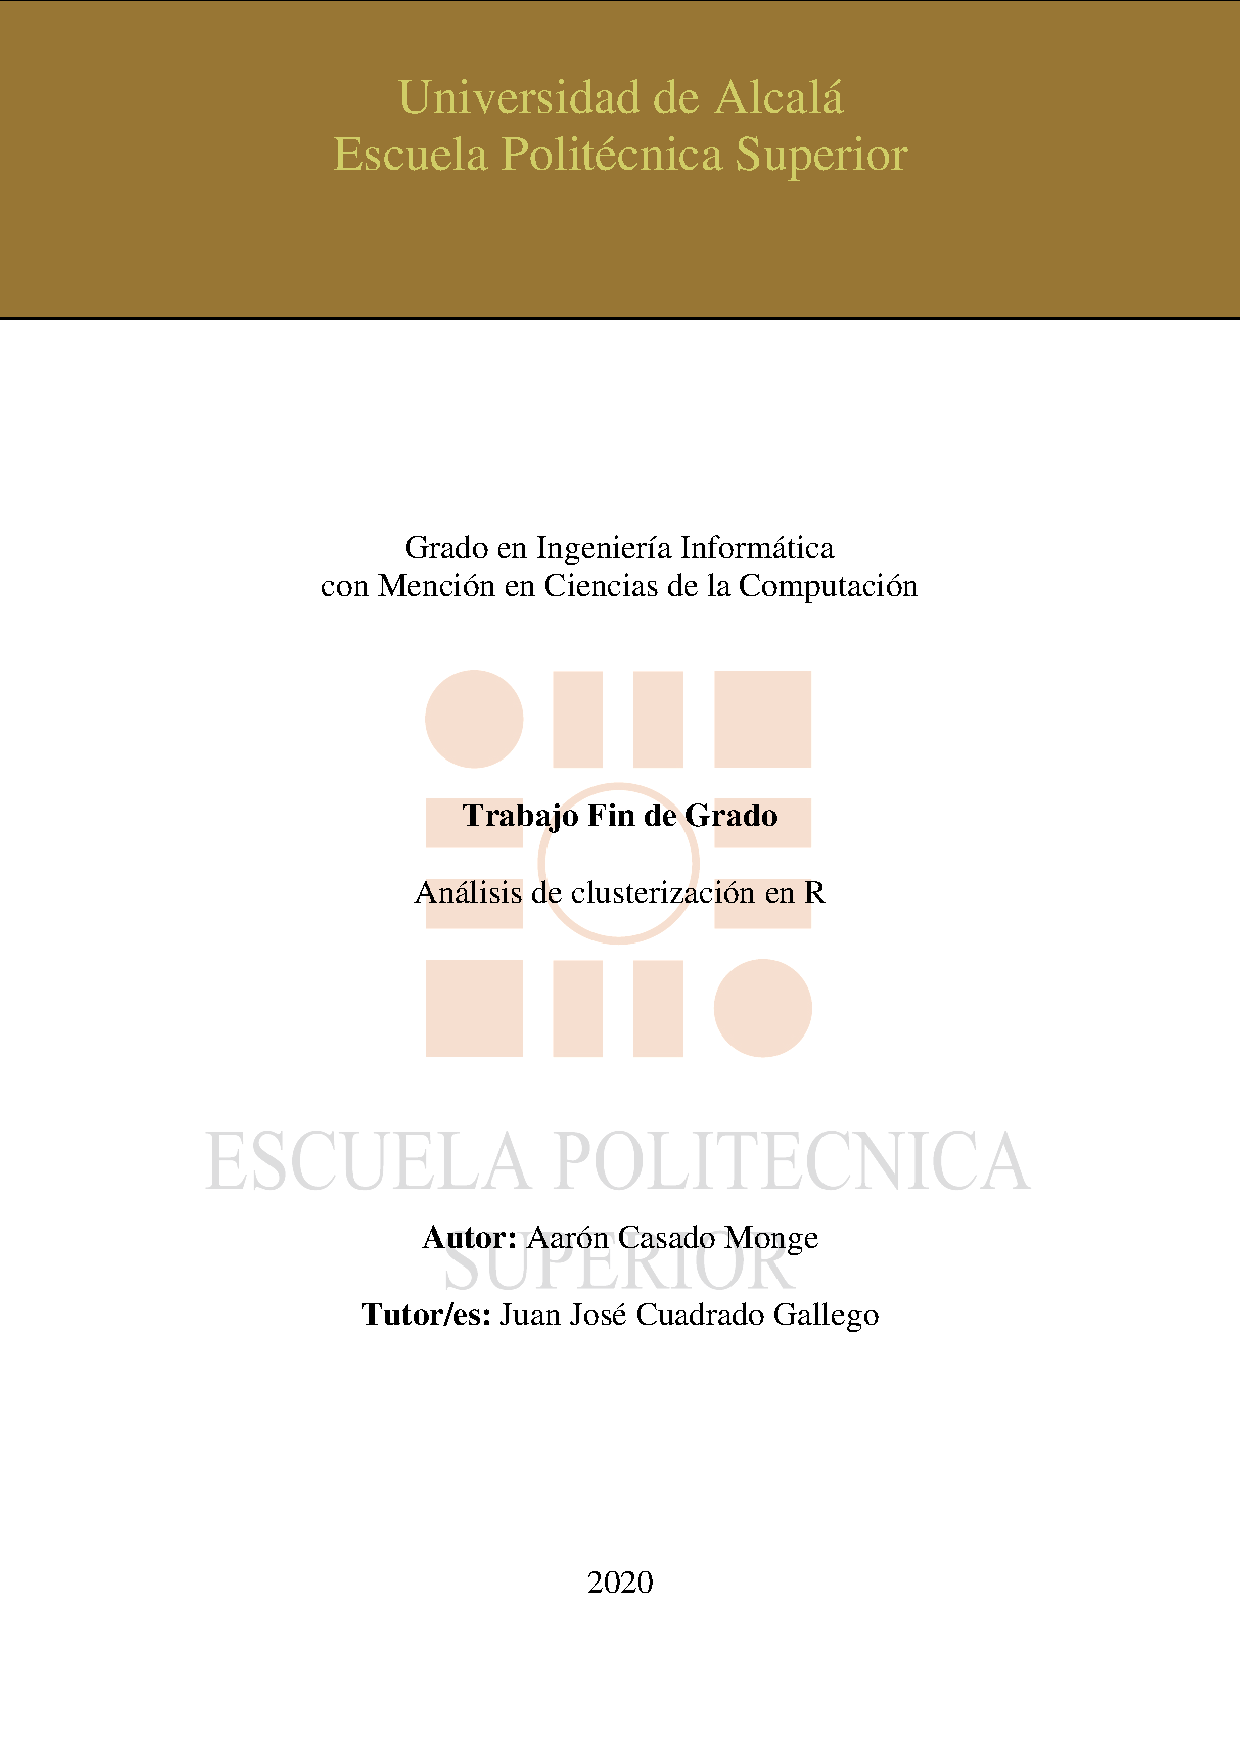
\includepdf[pages=1]{Recursos/portada.pdf}
    
    \title{Análisis de clustering en R}
    
    \author{Aarón Casado Monge$^{1}$, Juan José Cuadrado Gallego$^{1}$  \\
      \small $^{1}$University of Alcala, Polytechnic School, Computer Science Department, Scientific and Technological Campus, Politechnic Building. Office: O243, 28805, Alcala de Henares, Madrid, Spain}
  
    % Abstracto del TFG
    %\begin{abstract}{spanish}
    %    Clusterización
    %\end{abstract}
    
    %\selectlanguage{english}
    
    %\begin{abstract}
    %   Lo mismo pero en ingles.
    %\end{abstract}
    
    % Palabras clave del TFG
    %\keywords{Data Mining, Clustering, R}
    
  \maketitle
    
    
    \begin{center}
    \textbf{Resumen}
    \end{center}
    Resumen en español \newline
    \begin{center}
    \textbf{Abstract}
    \end{center}
    English abstract \\ \newline
    \textbf{Keywords}: Data Mining, Clustering, R. \newline
    
%====================================================================================================================================================%
                                              %============================================================%
%====================================================================================================================================================%

% Introducción del TFG
\section{Introducción}

Desde finales del sigo \textsc{xx} se ha considerado que vivimos en la ``era de la información'', una etapa caracterizada por el incremento, desarrollo y propagación de emergentes tecnologías de la información y comunicación que han permitido al ser humano romper las barreras de la distancia, el tiempo y el lugar a la hora de compartir información y comunicarse; actividades que han sido decisivas en nuestra historia \cite{INTRODUCCION}. Sin embargo, la era en la que realmente vivimos es la ``era de los datos'', donde cada día se generan más de veinticinco mil petabytes\footnote {Un Petabyte es una unidad de información o almacienamiento de datos equivalente a un cuadrillon de bytes, mil terabytes o un millón de gigabytes. En este caso, es el equivalente a 2.5 trillones de bytes.} de datos provenientes de comercios, ciencias, Internet y casi cualquier actividad del día a día \cite{DATA NEVER SLEEP} que acaban volcados en redes de ordenadores, sitios web, bases de datos y otros medios de almacenamiento. 

Esta explosión de datos, a la que se ha denominado Big Data, se debe al alto grado de computarización de la sociedad y el avance de herramientas de recolección y almacenamiento de datos. Negocios en todo el mundo generan grandes cantidades de datos derivados de transacciones, stock de productos,  platillas de empleados, etc. Las ramas de la ciencia producen datos de manera constante fruto de experimentos, observaciones, recogida de muestras, etc. Y más recientemente, Internet y las redes sociales han sido las principales responsables del aumento excesivo de datos, siendo usadas por millones de personas simultáneamente.

Y, aunque esto ha supuesto una considerable mejora para la humanidad, pues la información nunca había sido tan accesible y abundante, también ha ocasionado consecuencias negativas y problemas como el almacenamiento y organización de los datos, datos no estructurados que entorpecen su acceso y procesamiento, dificultades a la hora de analizar los datos apropiadamente pudiendo generar desinformación y complicaciones para mostrar los resultados de forma apropiada y aplicarlos de manera eficiente y útil en el mundo real \cite{3}.

Como resultado, ha surgido una nueva ciencia que se ha posicionado rápidamente como una de las disciplinas más influyentes de la actualidad: Data Science (Ciencia de los Datos), que debido a su reciente aparición, carece de una definición consensuada, pero podríamos concretarla como ``\textit{Ciencia que usa Estadística, Inteligencia Artificial, Programación y Bases de Datos para posibilitar la extracción de conocimiento a partir de datos}'' \cite{4}. A su vez, dentro de esta ciencia se han desarrollado otras tres ramas: Data Warehousing, Data Mining y Visualization; cada una de ellas enfocada a resolver o afrontar uno o varios de los problemas mencionados previamente: organización y agrupación de datos, análisis de los mismos y presentación de los resultados, respectivamente.

De entre estas nuevas disciplinas, Data Mining es la que se centra en el procesamiento de los datos, procedimiento por el cual se obtiene la información, y que se podría definir como ''\textit{Proceso de descubrimiento de patrones interesantes y conocimiento a partir de grandes volúmenes de datos}'' \cite{LIBRO}, donde dentro de la misma podemos encontrar diferentes técnicas para encontrar patrones y relaciones y dependiendo de cuál se aplique se puede obtener un resultado totalmente diferente incluso con el mismo conjunto de datos, por lo que es fundamental emplear la técnica apropiada en función del objetivo a conseguir, los datos con los que se pretende trabajar y el ámbito de aplicación.

Una de las numerosas formas con las que podemos obtener información de los datos es mediante la clasificación. Esta es una de las actividades más primitivas del ser humano y que ha sido fundamental en nuestro desarrollo, dado que en pos de entender un nuevo fenómeno o asimilar un nuevo objetos solemos buscar las características principales que lo defininen y compararlo con otros objetos o fenómenos conocidos en función de la similitud o disparidad que exista entre ellos. Este método comunmente aplicado en algunos de los campos más importantes del mundo moderno como la analítica de negocios, el reconocimiento de imágenes, las búsquedas web, seguridad, biología y ciencias de la salud. Sin embargo, existen dificultades a la hora de agrupar aquellos conjuntos de datos que no dispongan de una etiqueta o valor conocido que sirva como criterio de clasificación, ya sea porque dicho valor no existe o porque todavía no ha sido definido, y que son muy comunes en las disciplinas mencionadas previamente. 

Para poder clasificar este tipo de datos y afrontar este problema, se utiliza la técnica de \textit{clustering}, un método que precisamente permite generar valores y etiquetas para un determinado conjunto de datos realizando agrupaciones denominadas \textit{clusters} o grupos, donde los datos de un mismo cluster sean muy similares entre ellos y a su vez tengan diferencias claras con datos de otros clusters, permitiendo que cada grupo resultante pueda ser etiquetado y tratado como una clase propia, generando una clasificación de los datos que puede ser analizada y de la que se puede obtener conocimiento útil.

De esta manera, el objetivo de este Trabajo de Fin de Grado (TFG) es realizar un estudio sobre el método de clustering, exponiendo de manera teórica qué es este método y qué tipo de utilidades tiene, así como el desarrollo de las diferentes técnicas que existen y las aplicaciones que estas ofrecen. Posteriormente se explorará este método dentro de la Bioinformática, un campo centrado en desarrollar técnicas y programas software para analizar datos biológicos, viendo qué aporta a dicha disciplina y cuáles de las técnicas expuestas previamente se emplean y por qué. 

Una vez realizado el marco teórico previo, se pretende hacer una parte práctica en la que se analizarán los diferentes paquetes que ofrecen técnicas de clustering tanto de carácter general como dentro de Bioinformática para el lenguaje de programación R \cite{6}, uno de los más relevantes dentro de Data Science.


%====================================================================================================================================================%
                                              %============================================================%
%====================================================================================================================================================%


\section{Clustering} \label{clustering}

Clustering o cluster analysis, llamado en español agrupamiento o análisis de grupos y adaptado al término clusterización, es un método de Data Mining que se basa en el Aprendizaje Automático (Machine Learning), una rama de la Inteligencia Artificial (Artificial Intelligence) que pretende desarrollar sistemas que sean capaces de resolver problemas basándose en los resultados de experiencias previas, aprendiendo de sus errores. Concretamente, se fundamenta en uno de los métodos de aprendizaje explorados en esta disciplina: Aprendizaje No Supervisado, enfocado en el desarrollo y descubrimiento de nuevos conocimientos. Este, a diferencia de otros métodos de aprendizaje, no dispone de conocimiento o experiencias previas sobre las que poder aprender, por lo que su objetivo principal es discernir patrones y relaciones entre los datos para poder agruparlos y trabajar sobre los resultados de la clasificación resultante \cite{7}.

En esencia, el proceso de clustering es el mismo, hasta el punto en que básicamente podríamos considerarlos sinónimos, puesto que la clusterización se aplica principalmente sobre conjuntos de datos que se desean organizar en diferentes grupos pero los valores que delimitan cada cluster son desconocidos y por lo tanto se definen en el propio proceso de clasificación.

De una manera más técnica, podríamos decir que clustering busca definir para una determinada característica\footnote{Dicho de una cualidad que da carácter o sirve para distinguir a algo o alguien de sus semejante.} o Suceso Elemental\footnote{Cada uno de los resultados más simples que se pueen obtener de la realización de un experimento. Obtener el número 3 al tirar un dado.} (SE), un conjunto de grupos de observaciones (suceso) \footnote{Se denomina así al subconjunto total de resultados posibles al realizar un experimento. Obtener un 3 o sacar par al tirar un dado.} con valores cercanos, donde los clusters permiten, dados los diferentes sucesos elementales que configuran un suceso, asignar cada SE al mismo cluster \cite{8}.

Para poder decidir si dos datos deben ser agrupados en el mismo cluster o por el contrario, separados, es necesario introducir los conceptos de similitud y disparidad. Cuanto más similares sean los datos, más tendrán en común y por lo tanto es más probable que terminen bajo el mismo cluster; y por otra parte, si los datos son dispares entre sí, estos terminarán separados en clusters diferentes. Este criterio se basa en la proximidad de dichos objetos. Si midiéramos la similitud entre dos objetos \textit{i} y \textit{j}, esta devolvería 0 si ambos fueran totalmente distintos, y cuanto más elevado fuera el valor, más semejantes serían, siendo 1 el valor más alto, indicando que ambos datos son idénticos. De la misma manera, medir la disparidad entre los objetos daría resultados opuestos, con un 0 indicando que son idénticos y con un 1 que no tienen nada en común. 

Esta forma de calcular la proximidad no solo ayuda a la hora de agrupar los datos en clusters y formar subconjuntos a partir de los resultados, sino que con este proceso también somos capaces de detectar \textit{outliers}, datos anómalos que pueden ser datos erróneos procedentes de equivocaciones en mediciones o fallos que deben ser eliminados; o, datos correctos sumamente importantes que son diferentes al resto y deben ser analizados detenidamente. Podemos detectar este tipo de datos a la hora de agrupar los datos, pues puede que queden varios objetos sueltos sin pertenecer a ningún cluster, siendo esos los datos anómalos.

Además, clustering también sirve como primera aproximación a la hora de procesar los datos, porque aunque de por sí, este proceso puede aportar información útil agrupando datos similares y clasificándolos, permitiendo un análisis de los resultados que puede dar lugar al descubrimiento de nuevos conocimientos, también se usa como método de preprocesamiento de datos para otros algoritmos de Data Mining que trabajarán sobre los clusters generados y los atributos seleccionados como criterio a la hora de crearlos, considerando cada grupo resultante como una nueva clase de objetos.

Es gracias a estas características que la clusterización es empleada en muchos ámbitos del mundo actual, siendo la técnica de Aprendizaje No Supervisado más extendida. Campos como ingeniería (aprendizaje automático, inteligencia artificial, reconocimiento de imágenes), ciencias de la salud (genética, biología, microbiología, paleontología, psiquiatría, patología), ciencias sociales (sociología, psicología, educación) o economía (marketing, negocios) \cite{survey} hacen uso habitual de esta técnica para clasificar gran parte de los datos con los que trabajan y de los que se desconoce un atributo concreto por el que agruparlos. Dentro de estos sectores algunos de los ejemplos más comunes de clustering consisten en clasificar tipos de consumidores que comparten preferencias, aunar bajo un mismo subconjunto muchas formas diferentes de escribir el mismo caracter para facilitar el reconocimiento de textos escritos a mano, agrupar resultados similares de una consulta en internet y mostrar los más relevantes dentro de cada grupo o el estudio de la taxonomía\footnote{Ciencia que trata de los principios, métodos y fines de la clasificación. Se aplica en particular, dentro de la biología, para la ordenación jerarquizada y sistemática, con sus nombres, de los grupos de animales y de vegetales.} de las especies. 

También se puede hacer uso de su capacidad para detectar datos anómalos con la finalidad de revelar posibles fraudes o transacciones  financieras sospechosas, incluso ayudar en la disminución de crímenes analizando los resultados obtenidos tras clusterizar datos de detenciones y delitos; incluso aplicada a datos geofísicos\footnote{La Geofísica es la ciencia que estudia la Tierra desde el punto de vista de la física.} para interpretarlos y obtener resultados significativos. Asimismo, se utiliza a la hora de comparar comunidades en redes sociales permitiendo recomendar a los usuarios contenido de su agrado, o dentro del mundo sanitario, ayudando en la identificación y control de diversos tipos de enfermedades, e incluso puede usarse como apoyo en la gestión de edificios públicos como bibliotecas, agrupando a los lectores por sus preferencias de manera similar a los consumidores de un negocio \cite{9,10,11,12,13}.

Comprimiendo toda esta información, podemos concretar los tres principales objetivos por los que clustering es empleado: clasificación natural de individuos, objetos, etc., compresión de información para mayor facilidad a la hora de mostrar resultados y generación de una estructura base para el posterior tratamiento de los datos \cite{articulo14}.

La utilidad de este método y la flexibilidad que ofrece con las diversas técnicas y formas de aplicarlo de las que dispone es también parte fundamental de que sea tan comúnmente utilizado y con objetivos tan dispares en gran parte de las áreas del conocimiento. Sin embargo, también es un método frágil, pues depende en gran medida de los datos con los que se trabaje y el criterio escogido para determinar si dos objetos deben agruparse bajo el mismo cluster o separarlos, siendo necesario seguir una serie de pasos a la hora de realizar un análisis de grupos de manera correcta \cite{survey,15}:

\begin{enumerate}
  \item Primero, hay que seleccionar cuidadosamente los datos con los que se va a trabajar, puesto que tanto el tipo de dato como la cantidad de los mismos y el número de atributos\footnote{Dicho de una característica cualitativa de un individuo o dato usada para distinguirlo de una variable o característica cuantitativa.} influyen directamente en los resultados. Si se utilizan demasiados datos el procesamiento puede tener un coste computacional alto y es difícil ofrecer una visualización elegante de los resultados. Pero si se escogen pocos datos se pierde información útil y puede dar lugar a equivocaciones. Asimismo, datos con gran cantidad de atributos representan una dificultad añadida, elevando el coste computacional aún más y complicanto la toma de decisiones. Es por ello que este paso suele realizarlo un experto en el sector o con su ayuda. 
  
  \item Segundo, hay que optar por uno de los diversos algoritmos de clusterización que existen, pues los resultados pueden cambiar considerablemente al variar la estrategia con la que se realiza la agrupación. Este paso suele venir acompañado por la elección del procedimiento por el que se va a calcular la similitud entre los datos y clusters, y del criterio en el que se basa la decisión de agrupar en el mismo cluster dos datos. Esta última elección sinifica escoger el umbral de similitud a partir del cual dos datos pasan a formar parte del mismo cluster y qué característica o conjunto de ellas van a ser utilizadas para realizar la clasificación. La elección del umbral suele ser complicada, y es necesaria mucha experiencia o varias iteraciones de ensayo y error para encontrar un valor correcto. 
  
  \item Tercero, una vez generada la clasificación fruto del proceso de clustering es necesario validar el resultado obtenido, pues cualquier técnica de clusterización generará una agrupación de un conjunto de datos independientemente de si la solución aporta o no información útil. Es por ello necesario evaluar que la clusterización cumple con ciertos criterios y estandares para afirmar que el resultado es óptimo.
  
  \item Por último, una vez obtenidos los resultados hay que interpretarlos, pues el objetivo final de este proceso es aportar información útil de los datos analizados para resolver el problema inicial que ha llevado a este proceso. Este proceso suele ser realizado por expertos.
\end{enumerate}

\begin{figure}[ht]
\centering
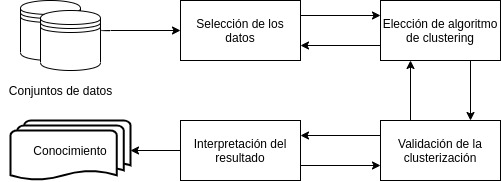
\includegraphics[width=\textwidth]{flowchart}
\caption{Procedimiento para el análisis de grupos. Este consta de cuatro pasos fundamenteales con realimentación \cite{survey}.}
\label{fig:flowchart}
\end{figure}

Como se puede aprecian el la figura \ref{fig:flowchart}, hay una vía de realimentación, pues la clusterización de los datos precisa de iteraciones de prueba y error, puesto que aunque la validación de la clusterización pueda aportar información acerca de la calidad del resultado, a veces es complicado encontrar el ajuste óptimo.

Asimismo, tanto el paso inicial como el último requieren de la ayuda de personas cualificadas si pretenden realizarse correctamente, y es en los pasos intermedios donde la intervención de computadoras y programas informáticos son más útiles y están más desarrollados, pues permiten aligerar considerablemente la carga de trabajo y como consecuencia, se puede analizar una mayor cantidad de datos. Pero no deja de ser una tarea complicada que ha ocasionado una gran demanda de expertos en Data Mining y Data Science en diversas áreas del conocimiento durante los últimos años.

La utilidad que aporta clustering permitiendo crear grupos con datos similares entre sí y dispares con respecto a otros grupos con el fin de clasificarlos y las ventajas que esto presenta queda reflejada en la cantidad de usos que recibe, por lo que vamos a profundizar en las diferentes técnicas que son empleadas para la generación de clusters que lo hacen tan importante.



%====================================================================================================================================================%
                                              %============================================================%
%====================================================================================================================================================%


\section{Técnicas de clustering} \label{sec:Técnicas de clustering}

Hay una gran variedad de técnicas de clustering que cumplen con el propósito de clasificar un conjunto de datos, pero no todas son iguales. Existen una serie de requisitos típicos que debe cumplir un algoritmo de clusterización para satisfacer las expectativas y realizar un buen análisis. Sin embargo, cumplir todos estos requerimientos de forma simultánea es una tarea casi imposible, haciendo que el desarrollo de nuevas técnicas y algoritmos o la modificación de los ya existentes sea constante. Analizar cuáles ofrece cada algoritmo nos ayuda a identificar sus puntos fuertes y débiles y por ende, facilitar la elección del algoritmo apropiado para cada ocasión. Veamos cuáles son dichos requisitos y qué criterios se usan para comparar algoritmos.

\subsection{\textbf{Requisitos de un algoritmo de clustering}} \label{subsec:Requisitos de un algoritmo de clustering}

\cite{LIBRO} El proceso de clustering es ubícuo siendo utilizado en gran cantidad de entornos, motivo por el que se han desarrollado numerosos algoritmos y técnicas orientadas a resolver diversos problemas en campos y disciplinas específicos. Sin embargo, no existe un algoritmo que pueda aplicarse uiversalmente a cualquier conjunto de datos y esperar que el resultado sea inmejorable. 

Existen trabas que complican este procedimiento tales como la cantidad de datos a analizar o el tipo de datos. Algunos de los algoritmos de clustering iniciales no tenían en cuenta este tipo de problemas, porque no existían en su momento, pero ahora es necesario afrontarlos para que el análisis de los datos sea eficiente y produzca resultados completos y veraces en cualquier circunstancia.

A continuación, se exponen los requisitos típicos que se exigen dentro de Data Mining a un algoritmo de clustering, así como debilidades que presentan algunos de los existentes, pues es imprescindible investigar el problema a tratar y saber escoger el algoritmo más adecuado para resolverlo.
 
\begin{itemize}
  \item \textbf{Escalabilidad}: Muchos algoritmos de clusterización trabajan bien con conjuntos de datos pequeños que contienen solo varios cientos de objetos; sin embargo, la gran mayoría de bases de datos contienen millones y miles de millones de datos. Analizar solo un pequeño porcentaje de esos datos puede resultar en conocimiento parcial. Que los algoritmos sean capaces de procesar pequeños y grándes volúmenes de datos es necesario para obtener resultados óptimos.
   
  \item \textbf{Habilidad para lidiar con diferentes tipos de atributos}: Coloquialmente se suele entiende por atributo un dato cuantitativo\footnote{Valor obtenido para una característica en una observación.}, es decir, un número. Sin embargo, existen otros tipos de datos: nominales\footnote{Dicho de un dato cualitativo que proporciona suficiente información para nombrar a una característica y poder diferenciarla de otra.}, binarios\footnote{Datos que solo pueden tomar los valores cero y uno (0, 1).}, ordinales\footnote{Datos cualitativos que proporcionan suficiente información para ordenar las observaciones.}, imágenes, gráficos, documentos y mezclas de varios de estos tipos. Por lo que un algoritmo de clustering debe estar preparado para trabajar con todos o la gran mayoría de ellos.
  
  \item \textbf{Descubrimiento de clusters con formas arbitrarias}: Gran parte de los algoritmos utilizan formas de calcular la similitud entre los datos basadas en la distancia entre los mismos, lo que suele dar lugar a clusters con formas redondas o esféricas. En determinadas ocasiones esto puede resultar contraproducente y erróneo, por lo que también es preciso que los algoritmos sean capaces de identificar diferentes formas de clusters, no solamente formas circulares o geométricas.
  
  \item \textbf{Requerir información al usuario}: En algunos algoritmos de clustering es común pedir cierto tipo de información al usuario a la hora de trabajar con los datos, como el número de clusters que se quieren generar. Este tipo de práctica puede ocasionar problemas dada la complejidad de esta decisión, sobre todo en escenarios en los que los datos cuentan con múltiples atributos. Por lo que es recomendable que los algoritmos eviten este comportamiento tanto para aliviar a los usuarios como para no comprometer la calidad a la hora de formar clusters, pues el algoritmo se adaptaría al valor introducido por el usuario, aunque fuese erróneo, generando también, un resultado errado.
  
  \item \textbf{Capacidad para trabajar con ruido en los datos}: Aunque es común tratar de antemano los datos para eliminar cualquier tipo de dato no deseado, recordemos que esta técnica también se aplica como método de preprocesamiento para otros algoritmos de Data Mining, por lo que es necesario que no sean sensibles hacia estas impurezas, puesto que podría resultar en una clasificación pobre. Asimismo, es posible que existan datos anómalos dentro de la muestra que pueden ser de gran utilidad y detectarlos es súmamente importante.
  
  \item \textbf{Clusterización incremental e insensibilidad al orden de entrada}: Cuando se aplica clustering en entornos en movimiento constante como el de los negocios, es común que se introduzcan datos nuevos junto a los ya existentes. Ciertos algoritmos no son compatibles con este incremento de información, y es necesario volver a iniciar un nuevo proceso de clusterización. Mientras que otros que sí toleran este cambio resulta que son sensibles al orden con el que se han introducido los datos y pueden generar agrupaciones erróneas. Estos problemas han dado lugar a la necesidad de algoritmos que puedan lidiar con la incorporación de nuevos datos y que no se vean afectados por el orden en el que estos son introducidos.
  
  \item \textbf{Capacidad de Clusterizar datos con muchos atributos}: Aunque de manera común se suele trabajar con datos que no contienen mucho más que una decena de atributos, hay ciertos tipos de datos como documentos, en los que cada palabra clave puede ser considerada un atributo, dando lugar a cientos de atributos por cada dato, haciendo complicado trabajar con ellos y también clasificarlos, haciendo necesarios algoritmos que puedan lograr un buen resultado con este tipo de datos.
  
  \item \textbf{Clustering basado en restricciones}: En el mundo real podemos encontrar ciertas barreras a la hora de aplicar un algoritmo de clustering, en los que, por ejemplo, sí se tenga que tener en cuenta un límite a la cantidad de clusters que se pueden generar o de decidir si dos datos o clusters deben unirse. Aunque es complicado realizar este tipo de agrupaciones, es indispensable que los algoritmos obtengan resultados decentes dadas estas limitaciones.
  
  \item \textbf{Interpretabilidad y usabilidad}: De nada sirve clasificar los datos y cumplir con los requisitos previos si no se puede interpretar el resultado. Los algoritmos, por lo tanto, deben ofrecer conclusiones comprensibles, coherentes y que puedan usarse, sometiéndose a ciertas limitaciones semánticas y visuales con la finalidad de acomodar el resultado al objetivo inicial por el que se ha llevado a cabo la clusterización que el usuario pueda enternder.
\end{itemize}


%====================================================================================================================================================%


\subsection{\textbf{Criterios de comparación}} \label{subsec:Criterios de comparación}

\cite{LIBRO} Cada algoritmo opera de forma distinta en diferentes aspectos como el criterio de división, la separación de clusters, el cálculo de la similitud y el espacio de clusterización. Observando los pasos a seguir y la toma de decisiones de un algoritmo, podemos compararlo con otro y escoger cuál es más adecuado para el problema a afrontar. 

\begin{itemize}
  \item \textbf{Criterio de división}: Principalmente existen dos tipos de métodos respecto a este criterio, aquellos que fraccionan todos los datos para que no exista ningún tipo de orden o diferencia de nivel entre ellos, y los que, por el lado opuesto, dividen los datos de manera jerárquica permitiendo formar clusters en diferentes niveles semánticos. Cada uno aporta una utilidad distinta, con el primer tipo de criterio podemos abordar problemas como la clasificación de clientes o lectores, conjuntos de datos en los todos reciben el mismo trato; mientras que con criterio de partición jerárquico podemos organizar documentos en varios campos como ``deportes'', ``política'' o ``comida'', y dentro de cada campo tener subconjuntos como ``postres'', ``pasta'' o ``carne''.
  
  \item \textbf{Separación de clusters}: Otro criterio en el que hay dos enfoques: si un dato forma parte de un cluster, este no puede formar parte de otro a no ser que ambos clusters se unan; o permitir que un dato pueda estar en dos clusters a la vez, un concepto denominado ``Fuzzy clustering''. La primera aproximación ofrece un enfoque más determinista que es quizás el más aplicado entre ambos métodos, pero existen disciplinas en las que permitir que un dato forme parte de más de un cluster, como se aprecia en la Figura \ref{fig:fuzzy}, puede ser realmente útil, por lo que cada vez recibe más usos \cite{17}. 
  
\begin{figure}[ht]
\centering
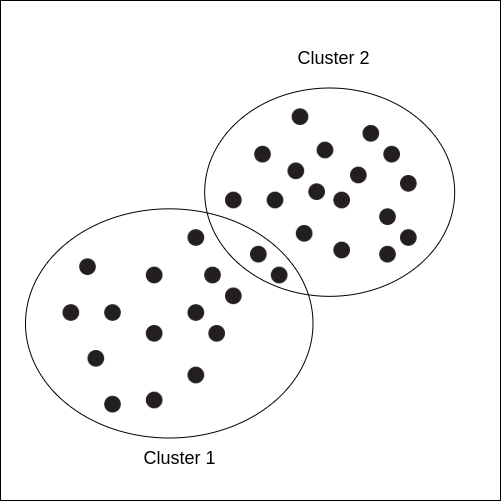
\includegraphics[width=0.5\textwidth]{fuzzy}
\caption{Fuzzy clusterering.}
\label{fig:fuzzy}
\end{figure}
  
  \item \textbf{Cálculo de similitud}: Una de las pautas que más determina un algoritmo de clusterización es la forma en la que calculan la similitud entre los datos, y que exploraremos detalladamente más adelante. Gran parte de los algoritmos utilizan la distancia que hay entre dos objetos para calcular su similitud aplicando métodos como la distancia Euclídea o espacios vectoriales. Este tipo de cálculo se ve beneficiado de métodos de optimización, pero suele generar clusters con formas esféricas o cilíndricas, por lo que cada vez más se utilizan algoritmos que miden la similitud entre objetos mediante la densidad o contigüidad del espacio para formar clusters, lo cual permite descubrir grupos con formas arbitrarias, aunque no son los únicos dos tipos.  
  
  \item \textbf{Espacio de clusterización}: Muchos algoritmos de clustering observan todo el espacio de datos para buscar grupos, que es un método totalmente factible y válido para datos con pocos atributos. Sin embargo, cuando se tratan de procesar datos con gran cantidad de atributos, es mejor centrarse en pequeñas partes del total, en subconjuntos del espacio de datos y buscar clusters dentro de ellos de forma que se pueda obtener información valiosa a un menor coste computacional.
\end{itemize}


%====================================================================================================================================================%


\subsection{\textbf{Clasificación general de técnicas}} \label{subsec:Clasificación general de técnicas}

\cite{LIBRO} Una vez que hemos visto los requisitos de los algoritmos de clustering y los criterios para compararlos entre sí, podemos agrupar la mayor parte de las técnicas bajo cuatro grandes grupos basados principalmente en el cálculo de la similitud y el criterio de división. Hablaremos brevemente sobre estos a continuación y posteriormente, precisaremos de manera individual sobre cada uno de ellos en las secciones \ref{sec:Métodos basados en particiones}, \ref{sec:Métodos jerárquicos}, \ref{sec:Métodos basados en densidad} y \ref{sec:Métodos basados en rejilla}, señalando los principales algoritmos dentro de cada una de ellos.

\begin{itemize}
  \item \textbf{Métodos basados en particiones}: Este tipo de métodos trata a cada objeto de manera equitativa situándolos a todos en el mismo nivel. Esto se consigue haciendo que en cada cluster haya al menos un objeto, es decir, si tenemos un conjunto de datos con $n$ objetos, los métodos basados en particiones generarán $k$ clusters siendo $k \leq n$. 

  
  Normalmente las técnicas de este grupo generan clusters exclusivos, donde un datos solo puede pertenecer a un cluster, pero cada vez se desarrollan más algoritmos de tipo fuzzy que relajan la agrupación. Asimismo, muchos de estos métodos calculan la proximidad entre los objetos como medida de similitud y generan de manera inicial $k$ particiones para posteriormente, de forma iterativa, tratar de reagrupar los datos y clusters para mejorar la clasificación, basándose en que los datos dentro del mismo cluster estén realmente cerca entre sí, y que con los datos de otros clusters se encuentren lejos.
  
  Estos métodos sirven tanto para búsquedas en todo el espacio de datos, como clusterización de espacios reducidos, pero cuando la cantidad de atributos es muy alta, es preferible utilizar esta segunda opción y aplicarlos en subconjuntos, pues es complicado optimizar computacionalmente este tipo de algoritmos a la hora de generar las particiones iniciales. Para lidiar con este inconveniente, se suelen usar métodos heurísticos como \textit{$k$-means} que intentan mejorar la calidad de clustering progresivamente. Sin embargo, como se ha mencionado previamente, esta aproximación de clustering genera grupos con formas esféricas y circulares, por lo que uno de los principales focos de mejora de estos algoritmos es evitar ese tipo de comportamiento cuando se trabaja con grandes conjuntos de datos.
  
  \item \textbf{Métodos jerárquicos}: Las técnicas de este grupo crean, como su propio nombre indica, una separación jerárquica de los datos. De forma diferente a los métodos basados en particiones donde todos los datos están en el mismo nivel, aquí se busca generar varios rangos para la clusterización. 
  
  Existen dos enfoques principales dependiendo de cómo se generen los clusters: \textit{aglomerativo} y \textit{divisivo}. Las técnicas aglomerativas parten de la separación de todos los objetos en clusters individuales que progresivamente se van uniendo hasta que solo queda uno; mientras que las técnicas divisivas parten de un solo cluster inicial en el que se encuentran todos los objetos y va formando clusters más pequeños hasta que cada objeto es en sí un cluster. Es por eso que también se les conoce por métodos de ``abajo a arriba'' y de ``arriba a abajo'' respectivamente.
  
  Esta técnicas pueden utilizar proximidad, densidad y continuidad como medida de calcular la similitud entre los datos y son útiles tanto en búsquedas de espacios completos como de subconjuntos.
  
  \item \textbf{Métodos basados en densidad}: Este tipo de métodos surgieron como solución a los métodos basados en particiones y su tendencia a encontrar únicamente clusters con formas esféricas o circulares, puesto que las técnicas que utilizan la densidad del espacio a la hora de formar clusters permiten descubrir clusters con formas más arbitrarias. 
  
  El concepto general de estos métodos consiste en agrandar un cluster mientras la densidad en el \textit{vecindario} esté por encima de un umbral. La densidad se calcula por la cantidad de objetos que hay en el espacio de datos y el vecindario hace referencia a todos los datos que se encuentran a cierta distancia de un objeto determinado.
  
  El concepto general es que para cada objeto dentro de un cluster, en su vecindario de radio $r$ de distancia debe haber un mínimo de $x$ objetos. Este tipo de aproximación resulta muy conveniente a la hora de detectar datos anómalos.
  
  Los métodos basados en densidad pueden clasificar los datos en clusters exclusivos o de manera jerárquica, y aunque normalmente consideran que un objeto solo puede pertenecer a un cluster, también existen técnicas de fuzzy clustering. Asimismo, se pueden aplicar tanto en espacios completos como en regiones puntuales.
  
  \item \textbf{Métodos basados en cuadrícula o rejilla}: Estos métodos dividen el espacio de objetos en una cantidad determinada de celdas que forman una estructura de cuadrícula o rejilla, de ahí su nombre. Todas las operaciones con los datos se realizan dentro de la rejilla, lo que permite un procesamiento mucho más rápido, pues no depende de la cantidad de datos, sino de la de celdas existentes.
  
  Esto permite que estos métodos puedan ser integrados con otros métodos de clustering pertenecientes a otros grupos como jerárquicos y basados en densidad para mejorar su eficiencia.
\end{itemize}

En la tabla \ref{Tab:Tabla 1} se han resumido estos grupos y las principales características de los mismos. Cabe mencionar que esta clasificación no es perfecta, pues existen algoritmos que integran conceptos de diferentes métodos.

Sin embargo, el mundo de Data Mining y de los datos no deja de crecer, implicando la aparición de nuevos tipos de problemas que afrontar con clustering. Esto ha dado lugar al desarrollo de nuevos algoritmos de clusterización que son lo suficientemente diferentes a los ya mencionados como para poder considerarlos otro tipo de métodos. Algunos de estos nuevos enfoques de clusterización se han convertido muy populares debido a sus nuevas características:

\begin{itemize}
  \item \textbf{Métodos de clusteriación relajada}: Como se ha mencionado previamente, lo más común a la hora de formar cluster es que estos sean exclusivos, es decir, que un objeto solo puede pertenecer a un cluster. Los métodos de clusterización relajada o fuzzy clustering  permiten que los objetos puedan estar en varios clusters a la vez. Esto se consigue utilizando el grado de pertenencia, un valor entre 0 y 1 que cuantifica la probabilidad o confianza de que un objeto pertenezca a un determinado cluster. La suma del grado de pertenencia de un objeto debe ser 1.
  
  Este enfoque es realmente útil cuando las fronteras entre los clusters no están separadas de una forma clara y es ambigua, puediendo además obtener más informacion gracias al grado de pertenencia. 
  
  Este tipo de métodos a veces se consideran modificaciones o variaciones de algoritmos, pero con la cantidad de atención y aplicaciones que ha recibido recientemente es adecuado tratarlos como un grupo distinto.
  
  \item \textbf{Métodos basados en modelos probabilísticos}: Uno de los objetivos de clustering es encontrar una estructura subyacente en los datos, algo oculto que no se vea a simple vista pero que esté latente en la muestra a analizar. Este tipo de métodos se aprovechan de esta característica para utilizar funciones de distribución y/o densidad como el origen de los datos a analizar, pues desde el punto de vista probabilistico, se asume que los objetos se generan de acuerdo a diversas distribuciones de probabilidad.
  
  Normalmente se utilizan distribuciones conocidas y estudiadas en profundidad como la Gausiana, eliminando así tener que buscar el modelo generativo y limitando la identificación de clusters a estimar los parámetros de dichas funciones probabilísticas.
  
  \item \textbf{Métodos basados en la teoría de grafos}: Podemos utilizar la teoría de grafos \cite{teoria grafos} para representar la clusterización mediante grafos ponderados, donde los nodos representan los objetos y las aristas que los conectan reflejan la proximidad entre pares de datos. 
  
  Para determinar los clusters se cortan las aristas más débiles, dejando juntos aquellos objetos que estén bien conectados entre sí, considerando esto un cluster, tal y como se aprecia en la Figura \ref{fig:grafo}, donde hay tres clusters claramente diferenciados por la falta de conexiones entre los objetos.
  
  Estos métodos surgieron como variante de los métodos jerárquicos y sirven tanto para clusterizar datos con muchos atributos o para analizar grafos per se.
  
  
\begin{figure}[ht]
\centering
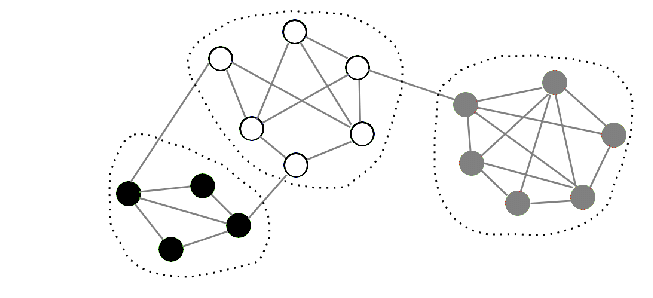
\includegraphics[width=0.8\textwidth]{grafo}
\caption{Clusterización basada en teoría de grafos \cite{foto grafo}.}
\label{fig:grafo}
\end{figure}
  
  \item \textbf{Métodos basados en redes neuronales}: Las redes neutonales artificiales son un área del aprendizaje automático que representan modelos matemáticos de la actividad cerebral. Su objetivo inicial era reproducir el procesamiento de información humano, y ahora este enfoque se ha aplicado en mucho campos, entre ellos clasificación. 
  
  Estos modelos consiste en un conjunto de unidades denominadas neuronas que están conectadas entre sí para trasmitir señales, de forma similar al cerebro humano. La información que recibe la red de forma inicial atraviesa las distintas neruonas donde se realizan ciertas operaciones y finaliza dando un valor de salida.
  
  Este tipo de métodos utilizan redes neuronales para localizar los clusters o en su defecto, sus centros, para facilitar el posterior desarrollo.
  
\end{itemize}

A continuación, exploraremos los cuatro primeros grupos (métodos basados en particiones, jerárquicos, basados en densidad y basados en rejilla), puesto que son los más populares y comunes, y tambien veremos los principales algoritmos empleados en cada uno de ellos y otros pertenecientes a los nuevos tipos de métodos.


\begin{table}[ht]
  \centering
  \resizebox{\linewidth}{!}{%
  \begin{tabular}{|l|l|}
    \hline
    \textbf{Métodos} & \textbf{Características generales} \\ \hline
    \begin{tabular}[c]{@{}l@{}}Basados en \\ particiones\end{tabular} & \begin{tabular}[c]{@{}l@{}}- Encuentran clusters de forma esférica mutuamente exclusivos\\ - Utilizan distancia/proximidad\\ - Usan la media o medoid para representar el centro del cluster\\ - Efectivos en conjuntos de datos pequeños y medianos\end{tabular} \\ \hline
    Jerárquicos & \begin{tabular}[c]{@{}l@{}}- Clasifican en múltiples niveles\\ - No pueden deshacer agrupaciones o divisiones erróneas\\ - Pueden incorporar otras técnicas como microclustering y tener en cuenta vínculos entre los objetos\end{tabular} \\ \hline
    \begin{tabular}[c]{@{}l@{}}Basados en \\ densidad\end{tabular} & \begin{tabular}[c]{@{}l@{}}- Pueden encontrar clusters con formas arbitrarias\\ - Los clusters son regiones con gran densidad de objetos separados por zonas con poca densidad\\ - La densidad queda definida por un mínimo de objetos cercanos dentro del vecindario\\ - Sirve para detectar datos anómalos\end{tabular} \\ \hline
    \begin{tabular}[c]{@{}l@{}}Basados \\ en rejilla\end{tabular} & \begin{tabular}[c]{@{}l@{}}- Utiliza una estructura de rejilla o cuadrícula\\ - La velocidad de procesamiento es alta, pues no influye el número de objetos\end{tabular} \\ \hline
    \end{tabular}%
  }
  \caption{Resumen de métodos de clusterización}
  \label{Tab:Tabla 1}
\end{table}


%====================================================================================================================================================%
                                              %============================================================%
%====================================================================================================================================================%

\section{Métodos basados en particiones} \label{sec:Métodos basados en particiones}

\cite{LIBRO} Los métodos pertenecientes a este grupo son quizás los más simples y básicos de clustering. Estos organizan los datos de un conjunto en diversos clusters exclusivos, y es común que soliciten al usuario el número de grupos o clusters finales que debe haber, lo que sirve como punto de partida . Esto permite simplificar su funcionamiento, pero a su vez, supone el incumplimiento de uno de los requisitos de los que se ha hablado previamente en la sección \ref{subsec:Requisitos de un algoritmo de clustering}.

De forma técnica, dado un conjunto de datos $D$ con $n$ objetos y siendo $k$ el número de clusters a formar, un algoritmo basado en particiones organizará los objetos en $k$ divisiones siendo $k \leq n$, donde cada una de ellas representa un cluster. 

Dichos clusters son generados intentando optimizar el criterio de similitud, siendo el del cálculo de proximidad uno de los más utilizados. Este intenta agrupar bajo el mismo cluster aquellos objetos que están cerca entre sí en el espacio de datos mientras hacen que todos los datos de un cluster estén alejados de los objetos de otro cluster, asegurando de esta manera un alto grado de semejanza entre los miembros del mismo cluster y de diferencia con los datos de otros clusters.

A continuación se exponen los dos algoritmos más utilizados de este grupo y de los más conocidos: $k$-media ($k$-means) \ref{subsec:k-means} y $k$-medoids \ref{subsec:k-medoids}.


%====================================================================================================================================================%


\subsection{\textbf{\textit{k}-Means}} \label{subsec:k-means}

El objetivo de los métodos basados en particiones es, dado un conjunto de datos $D$ con $n$ objetos en un espacio Euclídeo\footnote{Espacio geométrico donde se satisfacen los axiomas de Euclides.}, formar $k$ clusters, $C_{1}, ..., C_{k}$, donde cada cluster es un subconjunto del conjunto de datos $C_{i} \subset D$ y la intersección entre clusters es nula $C_{i} \cap C_{j} = \emptyset$ para $i \leq j$ y $j \leq k$. Sin embargo, estos requieren de una gran capacidad computacional, y es por ello que algoritmos como $k$-Means son tan utilizados, pues disminyen este coste.

$k$-Means representa cada cluster con su \textit{centroide}, que es básicamente el punto central del cluster y que se calcula como la media de los puntos que lo forman. Para un conjunto de datos con dos atributos cuantitativos, la fórmula para calcular el centroide $c_{i}$ es la siguiente: \begin{equation} c_{i} = \left( \frac{\sum _{i=1}^n x_{i}}{n}; \frac{\sum _{j=1}^m y_{j}}{m} \right). \end{equation} 

Asimismo, otro de los métodos más comunes para medir la distancia entre puntos y clusters, y que también utiliza $k$-Means, es la distancia Euclídea. La fórmula de la distancia Euclídea entre dos puntos cualesquiera $dist(p, q)$ de un espacio Euclídeo $p$ y $q$, con coordenadas cartesianas\footnote{Tipo de coordenadas ortogonales usadas en espacios Euclídeos que tienen como referencia los ejes ortogonales.} $(x_{1}, y_{1})$ y $(x_{2}, y_{2})$ es como sigue: \begin{equation}  dist\left( p,q\right) =  \sqrt{ \left(x_1-x_2 \right)^2 + \left(y_1 - y_2 \right)^2}. \end{equation} 

De esta manera, se utilizan sendas fórmulas para comprobar la calidad de un cluster y garantizar que los objetos del mismo sean similares entre ellos y diferentes con los objetos de otros clusters. Para ello, los métodos basados en particiones suelen utilizar la \textit{varianza} dentro del cluster, que es la suma del error cuadrático\footnote{Técnica para calcular la diferencia entre el estimador y lo que se estima.} entre todos los objetos del cluster $C_i$ y el centroide $c_i$, definida como: \begin{equation} E =  \sum_{i=1}^{k}  \sum_{p \in C_i} dist(p, c_i)^2 , \end{equation} donde $E$ es la suma del error cuadrático de todos los objetos pertenecientes al cluster $p_i \in C_i$. La finalidad de esta operación es asegurar que los $k$ cluster resultantes sean lo más compactos y distantes posible.

Es aquí, en el cálculo de la varianza donde la optimización de este método se vuelve computacionalmente complicada, pues en el peor de los casos, el total de posibles clasificaciones depende de manera exponencial del número total de clusters y posteriormente habría que comprobar los valores de la varianza dentro de cada cluster, siendo un problema de complexión NP-complejo\footnote{No se definir esto bien}. Para resolverlo, se utilizan algoritmos voraces\footnote{Estrategia de búsqueda en la que se sigue una heurística que consiste en escoger la opción más optima en cada paso de manera local, esperando llegar a una solución general óptima.} como $k$-Means, simples y usados habitualmente.

Este algoritmo sigue una serie de pasos para formar los clusters y evaluar su calidad. Primero, selecciona $n$ objetos dentro del conjunto de datos $D$ para representar los clusters iniciales; y puesto que son los únicos integrantes de ellos, el cálculo del centroide da como resultado el propio objeto. Posteriormente, asigna cada uno de los objetos restantes al cluster con el que es más similar basándose en el cálculo de la distancia Euclidiana entre el objeto y representante del cluster. A partir de aquí, el algoritmo intenta mejorar los resultados de la varianza, volviendo a calcular el centroide de cada cluster con los nuevos objetos añadidos en la iteración previa, y reagrupa los objetos ahora con los representantes de cada cluster actualizados. El proceso continua hasta que los centroides, y por ende, los clusters de la iteración actual sean idénticos a los de la iteración previa. El funcionamiento de $k$-Means queda reflejado en el Algoritmo \ref{alg:Algoritmo k-means} y ejemplificado en la Figura \ref{fig:kmeans}.

\begin{algorithm}[ht]
\SetAlgoLined
  \LinesNumbered
  \SetKwRepeat{Do}{repetir}{hasta}
  \DontPrintSemicolon
  \KwIn{$k$: número de clusters, \\ $D$: conjunto de datos con $n$ objetos.}
  \KwOut{Un conjunto de $k$ clusters.}
  \Begin{
    selección arbitraria de $k$ objetos de $D$ como representantes de los clusters iniciales\;
    \Do{no hay cambios}{
      calcular la distancia de cada objeto al centroide de cada cluster\;
      (re)asignar cada objeto al cluster con el que es más similar en función de la distancia obtenida\;
      actualizar los centroides de los clusters con los nuevos objetos añadidos\;
    }
  }
  \caption{$k$-Means, basado en la media}
  \label{alg:Algoritmo k-means}
\end{algorithm}


\begin{figure}[ht]
\centering
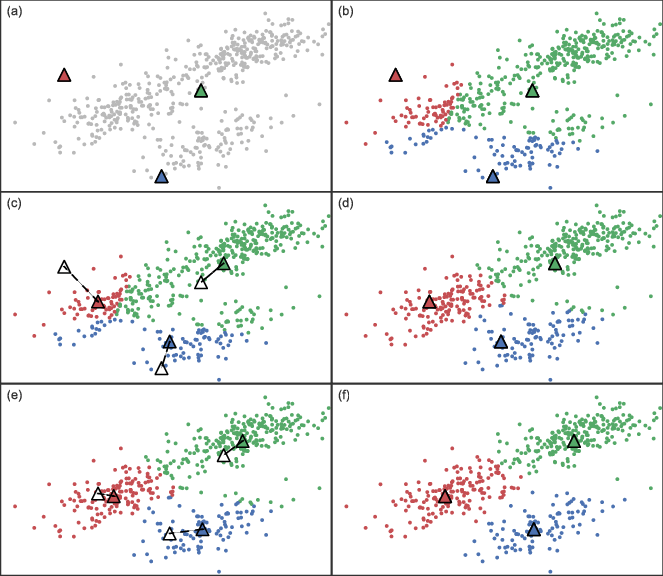
\includegraphics[width=\linewidth]{kmeans}
\caption{Ejemplo de $k$-means en dos dimensiones. (a) Los centroides de los clusters se inicializan en posiciones aleatorioas. (b) Primer paso: cada objeto se añade al cluster cuyo centroide es el mas cercano. (c) Segundo paso: Cada centroide se mueve a la media de los puntos que conforman el cluster. (d, e, f) Estos pasos se repiten hasta que el resultado de dos iteraciones sea el mismo. \cite{kmeansfoto}.}
\label{fig:kmeans}
\end{figure}


Sin embargo, este método no garantiza converger hacia un máximo global, sino que muchas veces termina en un máximo local por la utilización del algoritmo voraz. Esto hace que el resultado dependa de la selección de clusters iniciales sobre los que se trabaja, por lo que es es común realizar varias pruebas con diferentes clusters iniciales hasta encontrar un resultado óptimo. 

Por otro lado, la complejidad temporal de $k$-means es considerablemente baja  $O(nkt)$, pues depende del número de objetos $n$, del de clusters $k$ y de la cantidad de iteraciones $t$ y normalmente encontramos que $k \ll n$ y $t \ll n$. Lo cual sugiere que escalar este algoritmo a grandes conjuntos de datos es asequible.

Asimismo, este algoritmo solo puede ser utilizado cuando podemos calcular la media de los objetos para encontrar el centroide, por lo que en casos donde los datos tengan atributos nominales, no se puede aplicar de manera directa. Para ello existen modificaciones y versiones de $k$-means que solucionan algunos de estos problemas, como $k$-modas, que en vez de utilizar la media para calcular el centroide, utiliza la moda, el atributo que más se repite para una característica y si permite trabajar con datos nominales.

Otra de las desventajas que presenta y que comentábamos al inicio de la sección, es el hecho de que no cumple uno de los requisitos de los métodos de clustering, y es que $k$-means pide al usuario el número $k$ de clusters a generar como dato de entrada indispensable. Se han realizado estudios para solventar este problema intentando encontrar el mejor valor para $k$ ejecutando varias veces el algoritmo con distintos valores para esta medida, pero este paso extra supone un mayor coste computacional. 

Además, recordemos que este algoritmo flaquea a la hora de encontrar clusters con formas poco convencionales y de tamaños dispares, siendo realmente sensible a datos anómalos e impurezas, que pueden alterar los cálculos de los centroides y del resultado final.


%====================================================================================================================================================%

\subsection{\textbf
{Fuzzy \textit{k}-Means}}

Este algoritmo, también conocido como cuzzy $c$-means (FCM) \cite{fuzzymeans} es uno de los métodos de clusterización relajados más populares y utilizados \cite{otrolibro}. Utilizar algoritmos exclusivos en conjuntos de datos donde existen clusters superpuestos queda lejos de ser óptimo, por lo que aplicar una clusterización relajada es el método recomendado.

En FCM al igual que muchos otros métodos de clusterización relajada la pertenencia a diferentes clusters varía entre 0 y 1 y tiene un procedimiento similar al de $k$-means puesto que pretende reducir de forma iterativa el error cuadrático actualizando y modificando los valores del grado de pertenencia a los clusters utilizando los centroides de los mismos como representantes. El proceso termina cuando los centroides de una iteración no cambian con respecto a la anterior.

Al igual que $k$-means, este también es susceptible a las impurezas y datos anómalos de los datos. Muchos de los algoritmos de clusterización relajada se han basado en este para su desarrollo.



%====================================================================================================================================================%


\subsection{\textbf{\textit{k}-Medoids}} \label{subsec:k-medoids}

Como se ha mencionado en el apartado previo \ref{subsec:k-means}, $k$-means es realmente susceptible a datos anómalos e impurezas, pues como estos objetos se suelen encontrar alejados de todos los datos, cuando se asignan a un cluster y se recalcula el valor del centroide, este valor se ve altamente alterado, lo cual también afecta a la formación del resto de clusters.

Con el objetivo de ser menos sensible con estos datos, $k$-medoids utiliza uno de los objetos del cluster en vez de su centroide como representante del mismo, y el resto de objetos se añaden al cluster cuyo objeto representativo sea más similar. Por lo que el método para comprobar la calidad del cluster ya no es la varianza, sino el error absoluto, cuya fórmula es la siguiente: \begin{equation} \label{eq:k-medoids} E =  \sum_{i=1}^{k}  \sum_{ \in C_i} dist(p, o_i)^2 , \end{equation} siendo $E$ la suma del error absoluto de todos los puntos $p_i$ pertenecientes al cluster $C_i$ $\left(p_i \in C_i \right)$ con respecto al objeto representativo de dicho cluster $o_i$. De esta manera, $k$-medoids agrupa $n$ objetos en $k$ clusters minimizando el error absoluto. 

Los algoritmos más conocidos que utilizan esta aproximación para formar clusters son Partioning Around Medoids(PAM) y Clustering LARge Applications (CLARA), cada uno con sus propias características, que veremos a continuación.

%====================================================================================================================================================%

\subsubsection{\textbf{PAM}}

Este algoritmo, que podría traducirse al español como Particionamiento Sobre Medoids, es una de las aplicaciones más extendidas del método $k$-medoids, y tiene un funcionamiento similar a $k$-means en el sentido de que utiliza también una heurística voraz de forma iterativa para la formación de clusters y disminuir la complejidad computacional. 

Y de la misma forma, el paso inicial también es seleccionar de manera aleatoria $k$ objetos para formar los clusters iniciales, denominados ``semillas'', y asignar los objetos restantes al cluster cuyo objeto representativo (medoid) es el más similar. Posteriormente, con los nuevos clusters, se comprueba si cambiando el objeto representativo del cluster actual $o_i$ por otro objeto cualquiera dentro del cluster $o_{cualquiera}$ se mejora la calidad del cluster, y en caso de que sea así, se intercambia uno con otro. Esta comprobación se realiza para todos los objetos dentro del cluster que no sean el representante $o_{cualquiera} \neq o_i$ y para todos los clusters, hasta que no se pueda mejorar la situación actual. Una vez ha terminado este proceso, se vuelve a calcular la similitud entre todos los objetos y los representantes de los clusters y se reagrupan si es necesario. El algoritmo termina cuando los clusters resultantes de la iteración actual son idénticos a los de la previa. 

Para determinar la calidad del cluster y decidir si un representante del cluster debe ser cambiado por otro objeto dentro del cluster como se ha mencionado anteriormente, se calcula la distancia entre todos los puntos del cluster y su objeto representante actual $o_i$ mediante la fórmula \ref{eq:k-medoids}, cuyo resultado es almacenado. Luego, de forma iterativa cada objeto perteneciente al cluster se convierte en su representante $o_j$ temporal y se vuelve a calcular la distancia entre el resto de puntos y el representante temporal, y su resultado también se almacena, de forma que, una vez todos los puntos han sido representantes temporales y se ha aplicado la fórmula, se escoge como representante aquel objeto cuyo resultado ha sido el más bajo, es decir, el objeto más cercano a la mayoría de puntos del cluster, y si este nuevo punto es distinto al representante actual $o_i \neq o_j$, $o_j$ se convierte en el nuevo representante del cluster. 

Cuando un intercambio de representante ocurre en un cluster, se debe comprobar si es necesario reestructurar los clusters y el coste que esto conlleva, pues puede haber puntos cuyo cluster más cercano haya variado. Por lo que para cada punto del espacio de objetos se calcula la distancia a los nuevos representantes y se selecciona el que esté más cerca, pudiendo ser un nuevo cluster o el mismo en el que se encontraba pero con el nuevo representante. Una vez seleccionado el cluster más cercano para cada objeto, se calcula el coste con la misma función \ref{eq:k-medoids}, y si el resultado de esta reestructuración es negativo, es decir, si en la nueva situación los clusters representan mejor a los objetos porque el representante está más cerca de los puntos, se acepta este cambio y se considera que ha aumentado la calidad de los clusters.

\begin{algorithm}[ht]
\SetAlgoLined
  \LinesNumbered
  \SetKwRepeat{Do}{repetir}{hasta}
  \DontPrintSemicolon
  \KwIn{$k$: número de clusters, \\ $D$: conjunto de datos con $n$ objetos.}
  \KwOut{Un conjunto de $k$ clusters.}
  \Begin{
    selección arbitraria de $k$ objetos de $D$ como representantes $o_i$ de los clusters iniciales\;
    \Do{no hay cambios}{
      calcular la distancia de cada objeto al representante de cada cluster\;
      (re)asignar cada objeto al cluster con el que es más similar en función de la distancia obtenida\;
      seleccionar un objeto cualquiera del cluster que no sea el represente actual $o_{cualquiera}$\;
      calcular el coste $T$ de intercambiar el representante del cluster $o_i$ con $o_{cualquiera}$\;
      
      \uIf{T$<$0}{ intercambiar $o_i$ con $o_{cualquiera}$ como representante del cluster}
    }
  }
  \caption{PAM, basado en representantes}
  \label{alg:Algoritmo PAM}
\end{algorithm}

Este procedimiento, que queda reflejado en el algoritmo de PAM \ref{alg:Algoritmo PAM}, es más robusto que $k$-means al ser más tolerante a datos anómalos e impurezas, porque el medoid está menos influenciado por estos que la media. Sin embargo, esta aproximación es mucho más compleja computacionalmente para cada iteración, siendo esta $O \left(k\left(n-k\right)^2\right)$ y además, sigue solicitando el número de clusters $k$, por lo que para grandes volúmenes de datos resulta ineficiente, dando origen a otra versión enfocada precisamente a este tipo de trabajo: CLARA.


%====================================================================================================================================================%


\subsubsection{\textbf{CLARA}}

CLARA es una variación de PAM y que también aplica $k$-medoids a la hora de formar clusters, pero que en lugar de tener en cuenta todos los datos $n$ del conjunto de datos $D$, este algoritmo escoge una muestra aleatoria $m$ de datos y posteriormente aplica PAM para calcular los mejores representantes de la muestra. Esta muestra idealmente representa de una manera precisa al conjunto de datos original $D$ siempre y cuando cada objeto $p_i$ tenga las mismas posibilidades de ser escogido para la muestra. De esta manera y tras varias iteraciones seleccionando muestras arbitrarias, CLARA devuelve la mejor clusterización obtenida de todas ellas para aplicarla, ahora sí, en todo el conjunto de datos $D$.

Esto permite que la complejidad computacional disminuya, pues la comprobación de la calidad de los clusters y el intercambio de representantes que tanto costaba en PAM es reducido de manera drástica con este enfoque, permitiendo de esta manera que pueda trabajar con grandes volúmenes de datos. La complejidad para calcular los medoids de una muestra aleatoria es de $O\left(k\cdot s^2 + k\left(n - k \right)\right)$, siendo $s$ el tamaño de la muestra.

Sin embargo, este algoritmo depende totalmente de las muestras escogidas y la probabilidad de que el mejor representante de cada cluster se encuentre en ella, puesto que si tan solo uno de ellos no aparece en alguna de las muestras, CLARA nunca encontrará la mejor clusterización posible. 



%====================================================================================================================================================%
                                              %============================================================%
%====================================================================================================================================================%

\section{Métodos jerárquicos} \label{sec:Métodos jerárquicos}

\cite{LIBRO} Mientras que los métodos basados en particiones cumplen con el requisito básico de agrupar los datos en clusters exclusivos, hay ocasiones en las que clasificar los datos en diferentes niveles, es decir, de forma jerárquica, puede proporcionar grandes ventajas. De esta manera, los métodos jerárquicos organizan los datos en una jerarquía o árbol de clusters. 

Útil en escenarios donde los datos tengan de por sí cierta estructura jerárquica (\textit{p. ej.} estructura de empleados de una empresa) o en aquellos en los que se pretenda descubrir si existe una oculta(\textit{p. ej.} teoría de la evolución), estos métodos se clasifican a su vez en dos grupos: aglomerativos y divisivos. 

\begin{itemize}
  \item \textbf{Métodos jerárquicos aglomerativos}: Estos métodos utilizan una estrategia de ``abajo a arriba'', partiendo de que cada objeto compone su propio cluster, de forma iterativa los va uniendo en clusters más grandes hasta que solo queda un único cluster, que se conoce como ``raíz''. En cada iteración se mergen los dos clusters más cercanos entre sí para formar uno solo.

  \item \textbf{Métodos jerárquicos divisivos}: Este tipo de métodos utilizan una estrategia de ``arriba a abajo'', donde se sitúa a todos los objetos en un cluster inicial, la raíz, y de manera progresiva se divide la raíz en subclusters más pequeños sucesivamente hasta que cada cluster queda formado únicamente por un objeto o los objetos de cada cluster son prácticamente idénticos entre sí.
\end{itemize}

Como se puede ver, son métodos opuestos pero que operan bajo el mismo principio. Sin embargo, es mucho más complicado dividir los datos que juntarlos, pues hay muchas más posibilidades, en concreto, existen $2^{n-1}-1$ formas de dividir un conjunto de $n$ datos en dos clusters; por lo tanto, hay má muchas más comprobaciones que realizar, dando lugar a que los métodos aglomerativos sean más comunes y los divisivos dependan de métodos heurísticos que pueden dar resultados inexactos.

Los métodos jerárquicos pueden sufrir dificultades a la hora de dividir o juntar clusters, una parte crítica en su procedimiento, puesto que, a diferencia de los métodos basados en particiones donde en cada iteración se reagrupaban los puntos hacia el cluster más cercano, si un método jerárquico divide o junta dos clusters, no hay vuelta atrás y los siguiente pasos trabajarán con el resultado obtenido previamente sin poder cambiarlo. Por lo que decidir cómo y por qué motivo se genera un cluster es una tarea complicada y que de no ser correcta, puede ocasionar clasificaciones pobres. Otra desventaja principal de este enfoque es que no escalan bien hacia grandes volúmenes de datos, puesto que deben realizar muchas comprobaciones cuando se quieren unir o separar clusters aumentando exponencialmente el coste computacional.

Para lidiar con estos problemas se han desarrollado técnicas como BIRCH y Chameleon de las que se habla en las secciones \ref{subsec:BIRCH} y \ref{subsec:Chameleon}, que han resultado en otro tipo de clustering conocidos como multi fase y microclustering.

Antes de explicar algunos de los algoritmos más utilizados dentro de este grupo, AGNES \ref{subsec:AGNES}, DIANA \ref{subsec:DIANA}, BIRCH \ref{subsec:BIRCH} y Chameleon \ref{subsec:Chameleon}, analizaremos brevemente las diferentes maneras que existen en los métodos jerárquicos para medir distancias entre clusters.


%====================================================================================================================================================%


\subsection{\textbf{Medidas de distancia}} \label{subsec:Medidas de distancia}


Independientemente del tipo de método que se utilice, aglomerativo o divisivo, se necesita una forma de medir la distancia entre dos clusters.
Hay principalmente tres formas diferentes de realizar este cálculo como se puede apreciar en la figura \ref{fig:distancias}, aunque existen otras variaciones en las que, por ejemplo, se consideran los centroides como en $k$-means, estas utilizan puntos de clusters.

\begin{figure}[ht]
\centering
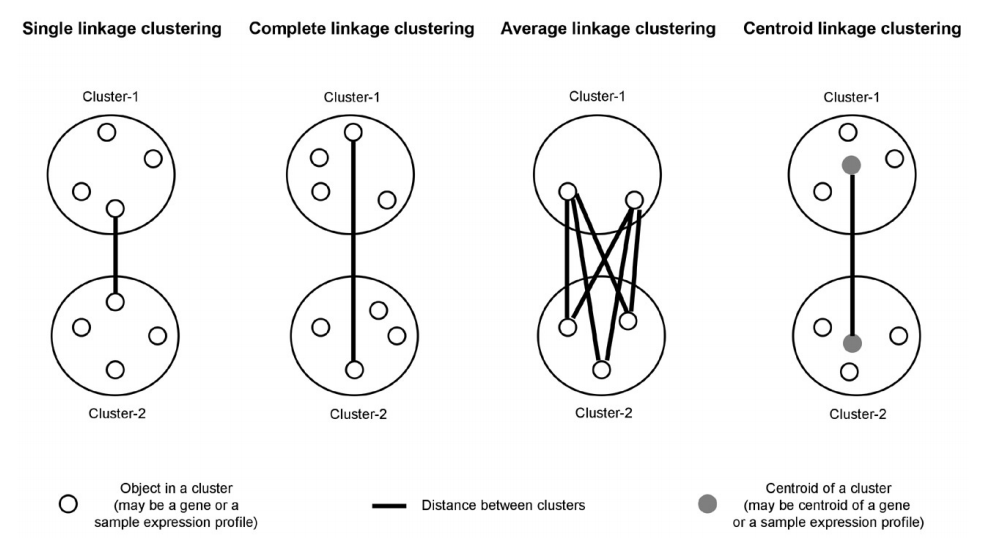
\includegraphics[width=\linewidth]{distancias}
\caption{Diferentes métodos para calcular la distancia entre clusters \cite{babu}.}
\label{fig:distancias}
\end{figure}


\begin{itemize}
  \item \textbf{Distancia mínima}: Esta define la proximidad entre dos clusters como la distancia entre los puntos más cercanos entre ambos, también conocida como ``single link''.
\begin{equation} dist_{min}(C_i, C_j) =  \min_{p \in C_i, p' \in C_j} \left\{|p - p'|\right\} \end{equation}

  \item \textbf{Distancia maxima}: Define la proximidad entre dos clusters como la distancia entre los puntos más alejados de ellos, también conocida como ``complete link''.
\begin{equation} dist_{max}(C_i, C_j) =  \max_{p \in C_i, p' \in C_j} \left\{|p - p'|\right\} \end{equation}

  \item \textbf{Distancia media}: Define la proximidad entre dos clusters como la distancia media entre todos los puntos de ambos clusters.
\begin{equation} dist_{avg}(C_i, C_j) = \frac{1}{n_i \cdot n_j} \sum_{p \in C_i, p' \in C_j} |p - p'|  \end{equation}
\end{itemize}

Las dos primeras son medidas que se van a los extremos y son susceptibles a datos anómalos e impurezas, por lo que el uso de la media es un compromiso entre ambas para solventar este problema.


%====================================================================================================================================================%


\subsection{\textbf{AGNES}} \label{subsec:AGNES}

\cite{jerarquico} AGglomerative NESting (AGNES) es quizás el algoritmo jerárquico aglomerativo más básico y extendido, pues aplica de forma exacta el concepto mencionado previamente. 

Parte de una separación de todos los objetos, cada uno formando un único cluster y compara la proximidad entre todos ellos utilizando el método que más convenga de los mencionados en la sección previa \ref{subsec:Medidas de distancia}. Selecciona aquellos dos con el resultado más pequeño, es decir, los dos más cercanos y los fusiona en un solo cluster, y se vuelven a calcular la similitud entre todos los clusters. Así sucesivamente hasta que todos los datos quedan agrupados en la raíz \cite{18}.


\begin{figure}[!ht]
\centering
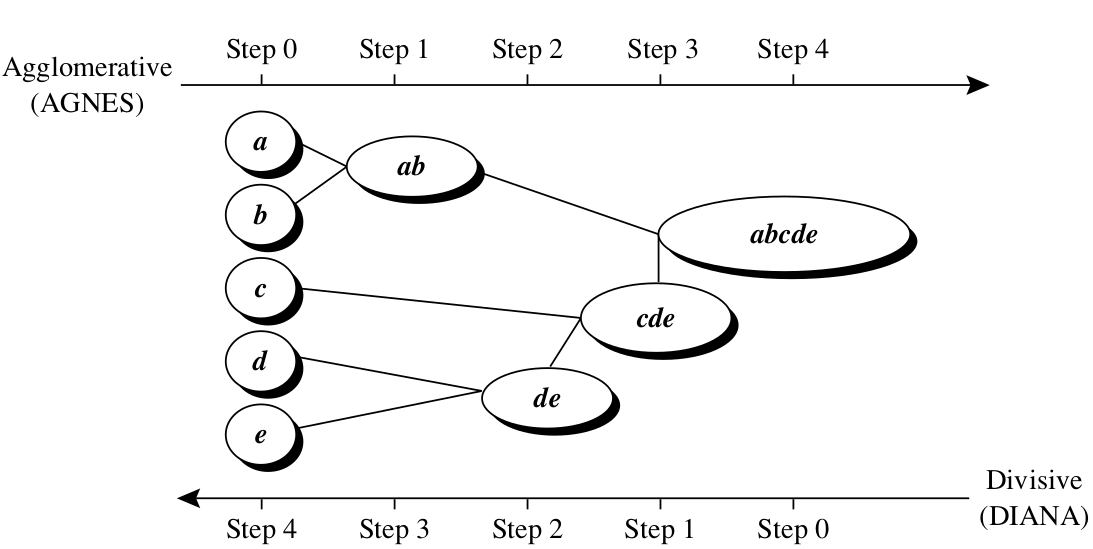
\includegraphics[width=0.9\textwidth]{dendograma}
\caption{Clusterización jerárquica algomerativa (AGNES) y divisiva (DIANA) sobre el conjunto de datos \{$a$,$b$,$c$,$d$,$e$\} \cite{LIBRO}.}
\label{fig:dendograma}
\end{figure}



%====================================================================================================================================================%


\subsection{\textbf{DIANA}} \label{subsec:DIANA}

\cite{jerarquico} El algoritmo DIvisive ANAlysis (DIANA) es la contraparte a AGNES, siendo también el método jerárquico divisivo más simple y utilizado. En este caso, al ser divisivo, parte de un solo cluster en el que se encuentran todos los datos y que de forma iterativa los va dividiendo en función de un criterio preestablecido, como por ejemplo la distancia Euclidiana mínima entre los objetos más cercanos del vecindario.

Tanto AGNES como DIANA generan una estructura denominada dendograma que se puede ver en la figura \ref{fig:dendograma}, donde se compara el proceso de estos dos algoritmos.


%====================================================================================================================================================%


\subsection{\textbf{BIRCH}} \label{subsec:BIRCH}

\cite{BIRCH, BIRCH 2} El algoritmo BIRCH, proveniente del nombre Balanced Iterative Reducing and Clustering using Hierarchies, es uno de los que mencionábamos previamente que combina el método jerárquico con otros métodos para solucionar los problemas de escalabilidad e imposibilidad de deshacer las divisiones o fusiones de clusters.

Para ello, BIRCH utiliza un concepto denominado \textit{característica de agrupamiento}, en inglés clustering feature (CF), que sirve para resumir un cluster, y otro llamado \textit{árbol de características de agrupamiento}, en inglés clustering feature tree (CF-tree), para representar la jerarquía de clusters. Estos dos atributos ayudan en la escalabilidad y rapidez del algoritmo y hacen posible utilizarlo en conjuntos de datos en los que se añaden nuevas muestras. Veamos brevemente cómo funciona.

Consideremos un cluster $C_i$ con $n$ objetos en él, CF es un vector de tres dimensiones que pretende resumir la información estadística del cluster de la siguiente manera \begin{equation} CF = \left(n, LS, SS \right ), \end{equation} donde $LS$ es la suma de los $n$ objetos y $SS$ es la suma de los $n$ objetos elevados al cuadrado. Esto permite obtener datos como el centroide $c_i$, el radio $R$ y diámetro $D$ del mismo, donde estos dos últimos representan lo ajustado que está el cluster alrededor del centroide. 

Usando esto, no hace falta guardar todos los datos del cluster, sino únicamente esta variable. Y a la hora de fusionar dos clusters $C_i$ y $C_j$, sus CF respectivos se suman tal que \begin{equation}CF_i + CF_j = \left (n_i + n_j, LS_i + LS_j, SS_i + SS_j \right ).\end{equation}

Por ejemplo, suponiendo que tenemos un cluster $C_i$ con los puntos (2,5), (3,2) y (4,3), $CF_i$ se calcula de la siguiente forma: 
\begin{align*}
n_i &= \left (3 \right), \\
LS_i &= \left (2 + 3 + 4, 5 + 2 + 3 \right) =  \left (9, 10 \right), \\
SS_i &= \left (2^2 + 3^2 + 4^2 , 5^2 + 2^2 + 3^2 \right) = \left (29, 38 \right), \\
CF_i &=  \left(n_i, LS_i, SS_i \right )= \left (3, \left (9, 10 \right), \left (29, 38 \right) \right).  
\end{align*}

Y si ahora, consideramos que hay que fusionar $C_i$ con $C_j$ para formar otro cluster nuevo $C_z$, siendo $CF_j = \left(3, \left(6,7 \right), \left(36,49 \right) \right)$, la operación sería la siguiente:

\begin{comment}
\begin{align*}
&CF_z = CF_i + CF_j =
&= \left(3, \left (9, 10 \right), \left (29, 38 \right) \right) +\left(3, \left(6,7 \right), \left(36,49 \right) \right)= \\
&= \left(6, \left(15,17 \right), \left(65,87 \right) \right).
\end{align*}
\end{comment}

$$CF_z = CF_i + CF_j = \left(3, \left (9, 10 \right), \left (29, 38 \right) \right) +\left(3, \left(6,7 \right), \left(36,49 \right) \right) = \left(6, \left(15,17 \right), \left(65,87 \right) \right).$$


El otro concepto que se ha mencionado previamente, CF-tree, tiene una estructura en forma de árbol que contiene el CF de cada cluster. Esta estructura de árbol, como se aprecia en la Figura \ref{fig:birch} está formada por nodos y hojas. Un nodo debe tener al menos un descendiente u hoja, mientras que las hojas son nodos terminales. Las hojas  almacenan el CF de un cluster, y su nodo padre o la raíz de dicha hoja almacena la suma de los CF de todos sus hijos. Este utiliza dos parámetros para controlar el desarrollo del árbol: el factor de ramificación $B$ y el umbral $T$ o $L$; estos indican cuántos hijos u hojas puede tener un nodo y cuántos nodos puede tener un cluster respectivamente. El tamaño del umbral determina el tamaño del árbol y su elección supone cierta dificultad. 

\begin{figure}[ht]
\centering
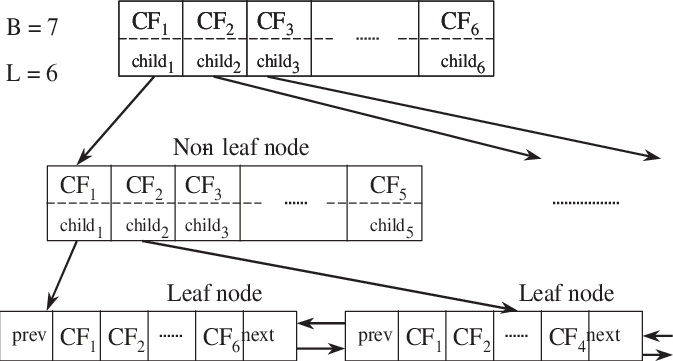
\includegraphics[width=\linewidth]{birch}
\caption{Estructura CF-tree del algoritmo BIRCH \cite{birchfoto}.}
\label{fig:birch}
\end{figure}

BIRCH es un método que consiste de dos fases principales, motivo por el que es considerado un algoritmo multifase:

\begin{enumerate}
  \item BIRCH escanea todo el conjunto de datos con la intención de formar un CF-tree inicial para comprimir todos los datos intentando mantener la estructura inherente de los datos. Esta fase es dinámica y el CF-tree es generado conforme se van insertando más datos, que se van añadiendo en las hojas siempre y cuando estas no superen ya el umbral $T$ de objetos permitidos, en cuyo caso, el cluster se divide en dos. Si llegase un punto en que tantos nodos no cupiesen en la memoria disponible, se aumenta el valor de T, permitiendo que los nodos alberguen más objetos y haya menos información que almacenar, provocando una reconstrucción de CF-tree.
  \item Posteriormente, se aplica un algoritmo de clusterización a las hojas del CF-tree que elimina clusters con poca calidad o pocos datos, que suelen ser datos anómalos y fusiona grupos de datos densos en clusters aún más grandes. Típicamente son algoritmos basados en particiones.
\end{enumerate}

Esta aproximación de clusterización ha probado ser rápida con una complejidad temporal de $O\left(n \right)$, escalable y fiable con los resultados generados, sin embargo sigue teniendo problemas puesto que el umbral $T$ determina en gran medida la formación de clusters y puede que se generen grupos que no son precisamente ``naturales'', y por otro lado, al utilizar el radio como criterio para definir clusters tiene peores resultados si los clusters no son esféricos o circulares.


%====================================================================================================================================================%


\subsection{\textbf{Chameleon}} \label{subsec:Chameleon}


\cite{chameleon} Chameleon es un algoritmo jerárquico y basado en grafos que utiliza un modelado dinámico para calcular la similitud entre pares de clusters. Esto es determinado por el grado de conexión entre los objetos dentro del cluster y la proximidad entre clusters; es decir, dos clusters se fusionarán si su interconectividad es alta y están muy cerca. Una de las principales ventajas de esta aproximación es que puede adaptarse a casi cualquier forma que pueda tomar un cluster para casi todos los tipos de datos, siempre que a estos se les pueda aplicar una función para calcular la similitud.

\begin{figure}[ht]
\centering
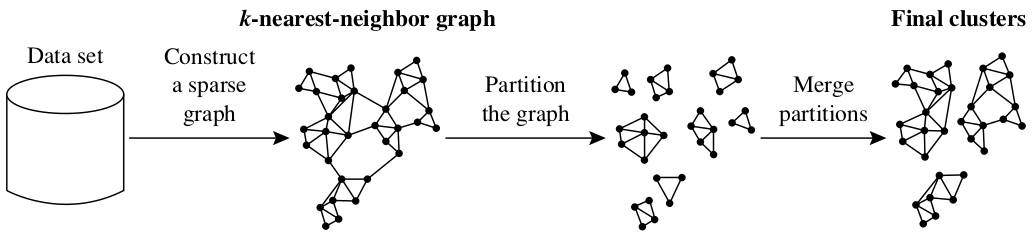
\includegraphics[width=\linewidth]{chameleon}
\caption{Chameleon: clusterización jerárquica basada en k-vecinos y modelado dinámico \cite{LIBRO}.}
\label{fig:chameleon}
\end{figure}

Este usa la aproximación de \textit{divide y vencerás}, donde primero particiona los datos en subclusters para posteriormente ir fusionándolos \cite{articulo14}.

En la imagen \ref{fig:chameleon} podemos observar el funcionamiento de este algoritmo. Primero utiliza $k$-vecinos para construir un grafo disperso, donde cada vértice representa un objeto y estos están conectados mediante aristas si dichos objetos se encuentran dentro del rango de $k$-vecinos y son similares. Las aristas, además, están ponderadas en función de la similitud de los objetos. 

Posteriormente, se aplica un algoritmo basado en particiones para dividir el grafo generado por $k$-vecinos en clusters, eliminando aquellas aristas con menos peso, es decir, las que unen clusters menos similares. Y una ver termina este proceso, se vuelve a aplica un algoritmo jerárquico aglomerativo que itera sobre los clusters generados y los fusiona basándose en la \textit{interconectividad relativa} y la \textit{cercanía relativa} de los clusters.

Este algoritmo ha demostrado ser capaz de identificar clusters con formas arbitrarias de mejor manera que otros algoritmos, pero su coste computacional sigue siendo elevado cuando se trabaja con conjuntos de datos con muchos atributos, siendo su complejidad $O\left(n^2\right)$.

%====================================================================================================================================================%


\subsection{\textbf{Métodos jerárquicos probabilísticos}} \label{subsec:Métodos jerárquicos probabilísticos}

Todos los métodos jerárquicos vistos hasta ahora utilizan algoritmos y medidas de proximidad para clusterizar, lo cual hace que sean fáciles de entender y eficientes en muchos ámbitos. Sin embargo, tienen varios problemas con los que todavía se intenta lidiar:

\begin{itemize}
  \item Establecer una distancia de proximidad para los métodos jerárquicos es complicado en la gran mayoría de los casos.
  \item Para aplicar un algoritmo, es necesario que los objetos tengan todos los atributos si se desea obtener un resultado de alta calidad.
  \item Muchos de estos métodos utilizan heurísticas que buscan optimizaciones locales fusionando o separando clusters, pudiendo resultar en un resultado global inexacto.
\end{itemize}

De esta manera, los métodos jerárquicos probabilísticos pretenden solventar algunos de estos problemas utilizando modelos probabilísticos para calcular la proximidad entre clusters tal.

Estos métodos, que también pertenecen al grupo de métodos basados en métodos probabilísticos de los que hablábamos al principio en la Sección \ref{subsec:Clasificación general de técnicas}, tratan de ver el conjunto de datos como el resultado de un mecanismo subyacente que ha generado los datos, denominado \textit{modelo generativo}, y lo que pretende esta forma de clustering es intentar estimar de la manera más precisa el modelo generativo a traves de los datos que se van a procesar. 

Normalmente se asume que estos modelos generativos siguen funciones de distribución como la de Bernoulli o la Gausiana, por lo que se reduce mucho el campo de trabajo y solo queda probar valores hasta dar con los que más se ajustan a los objetos del conjunto de datos. 


%====================================================================================================================================================%
                                              %============================================================%
%====================================================================================================================================================%

\section{Métodos basados en densidad} \label{sec:Métodos basados en densidad}


\cite{LIBRO} Los métodos jerárquicos y basados en particiones son muy útiles y eficaces encontrando clusters con formas esféricas y circulares, y aunque algunos de ellos sí puedan detectar en cierta medida otras formas, sigue siendo insuficiente en conjuntos de datos con datos anómalos e impurezas, donde es muy probable que no sean capaces de generar clusters de calidad.

Una solución a este problema es modelar los clusters como regiones densas de objetos separadas por regiones de baja densidad, la estrategia principal de los algoritmos basados en densidad. 

A continuación exploraremos los tres algoritmos más populares dentro de este grupo, DBSCAN \ref{subsec:dbscan}, OPTICS \ref{subsec:optics} y DENCLUE \ref{subsec:denclue}.

%====================================================================================================================================================%


\subsection{\textbf{DBSCAN}} \label{subsec:dbscan}


El algoritmo DBSCAN (Density-Based Spatial Clustering of Applications with Noise), propuesto por Martin Ester, Hans-Peter Kriegel, Jorg Sander y Xiaowei Xu en 1996 \cite{DBSCAN}, se basa fundamentalmente en encontrar los objetos en cuyos alrededores haya más puntos y conectarlos con aquellos de iguales características para formar clusters, dejando como separación entre ellos áreas con pocos datos.

Este algoritmo solicita dos valores al usuario, el primero \textit{Espsilon} $\epsilon > 0$ delimita el radio del vecindario de todos los objetos, y el segundo \textit{MinPts} es utilizado para determinar la densidad del vecindario de un objeto $o$. Cuando el vecindario de un objeto $o$, definido como $N_{\epsilon}(o) = \{o \in D | dist(o,q) \leq \epsilon\}$, contiene más de \textit{MinPts} objetos, $o$ se considera un objeto central o núcleo, que es el centro o pilar de un cluster.

Sin embargo, si solo utilizáramos esto para formar los clusters, tendríamos problemas con interferencias y datos anómalos, pues los puntos en los bordes tienen menos objetos a su alrededor y se podría dar al cluster una forma errónea. Para evitar eso, se requiere que, para cada punto $p$ de un cluster $C$, haya otro punto $q$ en $C$ tal que $p$ esté dentro del vecindario de $q$ ($p  \in N_{\epsilon}(q)$) y que en el vecindario de $q$ haya al menos $MinPts$ objetos ($N_{\epsilon}(q) > MinPts$). Si se cumple esta condición, se considera que $p$ es \textit{directamente alcanzable por densidad} desde $q$.

Esta condición suele ser recíproca entre núcleos, pero no entre núcleos y puntos fronterizos, tal y como se aprecia en la figura \ref{fig:dbscan1}

\begin{figure}[ht]
\centering
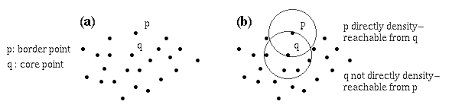
\includegraphics[width=\linewidth]{dbscan1}
\caption{DBSCAN: diferencia entre núcleos y puntos fronterizos \cite{DBSCAN}.}
\label{fig:dbscan1}
\end{figure}

De esta definición se puede extrapolar otra, y es que un punto $p$ es \textit{alcanzable por densidad} desde $q$, si hay una cadena de puntos $p_1, \cdots, p_n$ donde el primer punto es $q$ ($p_1 = q$) y cada punto sucesivo $p_{i+1}$ es directamente alcanzable por densidad desde el anterior $p_i$. Al igual que la anterior, no suele ser recíproca con núcleos y puntos fronterizos, pero sí entre núcleos. Sin embargo, puede que existan dos puntos fronterizos del mismo cluster que no sean alcanzables por densidad entre ellos porque no tengan $MinPts$ objetos en su vecindario, pero que si lo sean desde un núcleo del cluster, que da lugar a otra definición.
 
Se dice que un punto $p$ está \textit{conectado por densidad} a un punto $q$ si hay otro punto $o$ desde el cuál, ambos, $p$ y $q$, son alcanzables por densidad, y esta propiedad si es recíproca siempre.  

Ejemplos de estas tres definiciones pueden observarse en la figura \ref{fig:dbscan2}.

\begin{figure}[ht]
\centering
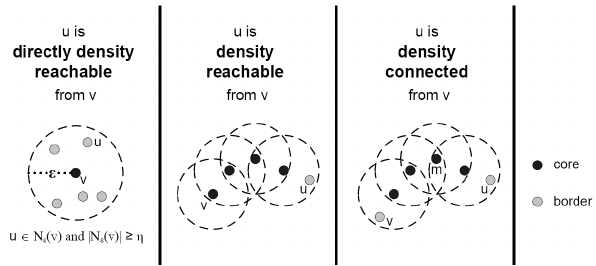
\includegraphics[width=\linewidth]{dbscan2}
\caption{DBSCAN: términos \textit{directamente alcanzable por densidad}, \textit{alcanzable por densidad} y \textit{conectado por densidad} \cite{DBSCAN 2}.}
\label{fig:dbscan2}
\end{figure}

Con estos conceptos, DBSCAN es capaz de formar clusters de forma que todos sus objetos estén conectados por densidad y detectando como impurezas y datos anómalos aquellos puntos que no pertenezcan a ningún cluster.

Así pues, el primer paso de este algoritmo es seleccionar un punto cualquiera $p$ del conjunto de datos $D$, y comprueba todos los puntos alcanzables por densidad con respecto a $\epsilon$ y $MinPts$. Si $p$ es un núcleo, se forma un cluster con todos los objetos alcanzables por densidad desde $p$ que no pertenezcan a otro cluster, y si es un punto fronterizo, no hay puntos que sean alcanzables por densidad desde $p$, por lo que es marcado como ruido y selecciona otro objeto. 

Una vez ser forma el cluster, se selecciona otro objeto que no se haya visitado y se repite la operación. Asimismo, DBSCAN puede fusionar dos cluster si se encuentran muy cerca entre sí. Este procedimiento queda reflejado en el algoritmo \ref{alg:Algoritmo DBSCAN}.



\begin{algorithm}[!ht]
\SetAlgoLined
  \LinesNumbered
  \SetKwRepeat{Do}{repetir}{hasta}
  \DontPrintSemicolon
  \KwIn{$D$: conjunto de datos con $n$ objetos, \\$\epsilon$: radio del vecindario, \\ $MinPts$: umbral de densidad del vecindario.}
  \KwOut{Un conjunto de clusters basados en densidad.}
  \Begin{
    marcar todos los objetos como no visitados\;
    \Do{quden objetos por visitar}{
      seleccionar un objeto $p$ no visitado\;
      marcar $p$ como visitado\;
      \uIf{el $\epsilon$ vecindario de $p$ tiene al menos $MinPts$ objetos}{
          creamos un nuevo cluster $C$ y le añadimos $p$\;
          sea $N$ el conjunto de objetos en el $\epsilon$ vecindario de $p$\;
          \ForEach{punto $p' \in N$}{
            \uIf{$p'$ no ha sido visitado}{
              marcamos $p'$ como visitado\;
              \uIf{el vecindario de $p'$ tiene al menos $MinPts$}{añadimos los puntos del vecindario de $p'$ a $N$}
              \uIf{$p'$ no pertenece a ningún cluster}{añadimos $p'$ a $C$}
            }
          }
          devolvemos $C$\;
        }
        \uElse{marcamos $p$ como ruido}
      }
  }
  \caption{DBSCAN, basado en densidad}
  \label{alg:Algoritmo DBSCAN}
\end{algorithm}


%====================================================================================================================================================%


\subsection{\textbf{OPTICS}} \label{subsec:optics}

Sin embargo, DBSACN sigue solicitando al usuario $\epsilon$ y $MinPts$, valores cruciales en la formación de clusters y de difícil elección que incumplen uno de los requisitos de los algoritmos de clustering vistos en la sección \ref{subsec:Requisitos de un algoritmo de clustering}. Como solución a este problema y sin la necesidad de introducir parámetros de entrada, surgió OPTICS (Ordering Points to Identify the Clustering Structure), que no devuelve una clusterización, sino un orden de clusters (cluster ordering); una lista lineal de todos los objetos del conjunto de datos que representa la estructura de clusterización basada en la densidad de los datos. Aquellos objetos que sean próximos entre sí estarán más cerca en la lista de ordenación.

Con este proceso podemos extraer la información básica de la clasificación, como los centros de los clusters o grupos con formas raras, una visualización de la clusterización y también se puede derivar la estructura intrínseca de la agrupación.

Para ello, OPTICS necesita obtener dos datos adicionales para cada objeto, cuyos conceptos se reflejan en la Figura \ref{fig:optics}:

\begin{itemize}
  \item \textbf{Distancia al núcleo}: La \textit{distancia al núcleo} de un objeto $p$ es el valor más pequeño para $\epsilon'$ de manera que en el vecindario delimitado por dicho valor haya al menos $MinPts$, y si $p$ cumple con esta condición, se le considera núcleo. En caso de que que no haya $MinPts$ en el $\epsilon'$ vecindario, se considera que la distancia al núcleo es indefinida.
  
  \item \textbf{Distancia de alcance}: La \textit{distancia de alcance} hacia un objeto $p$ desde otro objeto $q$ es el radio mínimo que hace que $p$ sea alcanzable por densidad desde $q$ (\ref{subsec:dbscan}), por lo que $q$ debe ser un núcleo y $p$ debe estar en su vecindario. Si $q$ no es un núcleo, se considera que la distancia de alcance de $p$ a $q$ es indefinida. 
  
  Es posible que un objeto $p$ tenga más de una distancia de alcance, es decir, que sea alcanzable desde varios puntos. En este caso, la medida que más nos interesa es la distancia de alcance más pequeña. Se puede formalizar el concepto de distancia de alcance como $\max\{distancia \ al \ nucleo(q), dist(p,q)\}$. 
\end{itemize}

\begin{figure}[ht]
\centering
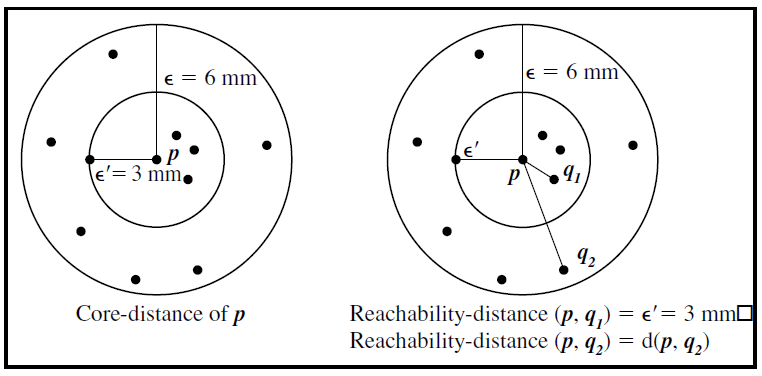
\includegraphics[width=\linewidth]{optics}
\caption{OPTICS: conceptos de distancia al núcleo (core-distance) y distancia de alcance (reachability-distance).}
\label{fig:optics}
\end{figure}

OPTICS almacena para cada objeto del conjunto de datos la distancia al núcleo y una distancia de alcance apta, y en función de la distancia de alcance de cada objeto desde su núcleo más cercano, genera una lista llamada OrdenSemillas (OrderSeeds). 

Posteriormente, se escoge un objeto cualquiera como punto actual $p$ del que se obtiene su $\epsilon$ vecindario y se calcula su distancia al núcleo, estableciendo a priori su distancia de alcance como indefinida. Si $p$ no es un núcleo, simplemente se pasa al siguiente objeto de OrdenSemillas, pero si $p$ es un núcleo, se actualiza la distancia de alcance para cada objeto $q$ de su $\epsilon$ vecindario y se inserta en OrdenSemillas si todavía no está en la lista. Esta iteración continúa hasta que la lista OrdenSemillas está vacía. 

Tanto DBSCAN como OPTICS tienen una complejidad de $O\left(n^2\right)$ para $n$ número de objetos.


%====================================================================================================================================================%


\subsection{\textbf{DENCLUE}} \label{subsec:denclue}

Los dos algoritmos previos, DBSACN y OPTICS (\ref{subsec:dbscan}, \ref{subsec:optics}) presentan un inconveniente, $\epsilon$. Pequeñas variaciones en el radio del vecindario de los objetos puede resultar en clusters totalmente distintos. DENCLUE \cite{DENCLUE} (DENsity based CLUstEring) pretende solventar este problema utilizando un enfoque de estimación de densidad no paramétrica llamado \textit{estimación de densidad nuclear}.

el concepto principal detrás de este algoritmo está basado en la idea de que la influencia de cada punto, es decir, el impacto que este tiene en su vecindario, puede ser modelada formalmente utilizando una función matemática denominada \textit{función de influencia}, con la que podemos obtener la densidad media del espacio de datos sumando  la función de influencia de todos los puntos.

De esta manera, los clusters pueden ser formados encontrando los denominados \textit{atractores de densidad}, puntos locales máximos de la función de densidad media. Estos se pueden hallar mediante el algoritmo de Escalada Simple\footnote{Técnica de optimización matemática utilizada para encontrar óptimos locales.} guiado por el gradiente de la propia función. El uso de la función de densidad media también facilita encontrar clusters de formas arbitrarias.

DENCLUE implementa de manera eficaz este planteamiento y lo hace más eficaz, pues no todos los puntos del espacio de datos contribuyen de forma notable en la función de densidad media, por lo que en su lugar, usa una función local de densidad, teniendo en cuenta solo aquellos puntos que influyen en la función. En el primer paso de este algoritmo, se preprocesan los datos, generando un mapa de los objetos relevantes del espacio de datos que sirve para aumentar la velocidad de cálculo de la función de densidad. El segundo paso es el propio clustering, donde se identifican los atractores de densidad y todos los puntos a los que estos influyen.

Este algoritmo tiene varias ventajas, y es que es tan versátil como otros algoritmos como DBSACN y $k$-means, pero además tolera extremadamente bien datos anómalos e impurezas.


%====================================================================================================================================================%
                                              %============================================================%
%====================================================================================================================================================%


\section{Métodos basados en rejilla} \label{sec:Métodos basados en rejilla}

\cite{LIBRO} Todos los métodos expuestos hasta ahora tienen se enfocan principalmente en los datos, es decir, se basan en la distribución de los objetos en el espacio de datos para formar los clusters. Sin embargo, los métodos basados en rejilla se centran en el propio espacio; no dividen los datos, sino el espacio de datos, que distribuyen en celdas equitativas, independientemente de cómo estén repartidos los puntos.

Estos métodos dividen el espacio de datos en un número finito de celdas que forman una estructura de rejilla o cuadrícula, donde se realizan las operaciones de clusterización, aumentando considerablemente la velocidad de clustering, hasta el punto que la cantidad de datos es irrelevante y solo depende del número de celdas. Es esta característica lo que hace estos métodos ideales para combinarlos con otro tipo de métodos y mejorar su eficiencia.

En esta sección veremos dos de los métodos más conocidos dentro de este grupo, STING \ref{subsec:sting} y CLIQUE \ref{subsec:clique}.


%====================================================================================================================================================%


\subsection{\textbf{STING}} \label{subsec:sting}

\cite{sting} STING (STatistical INformation Grid) es una técnica de clusterización en la que el espacio de datos es dividido en celdas rectangulares o cuadradas, con la opción de poder descomponerlo de forma jerárquica. Cada capa de celdas forma un nivel distinto, done cada celda de un nivel superior está compuesta por varias celdas del nivel inferior, lo cual permite obtener esa estructura jerárquica de los datos tal y como se aprecia en la Figura \ref{fig:sting}.

\begin{figure}[ht]
\centering
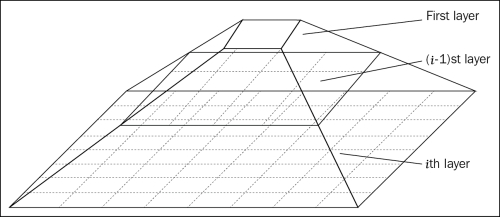
\includegraphics[width=\linewidth]{sting}
\caption{STING: división del espacio de datos en celdas en diferentes niveles \cite{sting 2}.}
\label{fig:sting}
\end{figure}

De cada celda se calcula de antemano información estadística clave de los datos que esta contiene, tales como la media, máximo, mínimo; lo que facilita la obtención de paramentos para las celdas superiores: el número de objetos dentro de la celda, la media, desviación típica\footnote{Medida estadística que sirve para cuatificar la dispersión de un conjunto de datos numéricos.}, máximo, mínimo y si los datos siguen algún tipo de distribución (normal, uniforme, exponencial o ninguna). 

STING selecciona una de las capas superiores que se han generado, no necesariamente la primera, sino una con pocas celdas; examina todas ellas y descarta aquella celdas que tras analizarlas, se considere que tienen poca relevancia con respecto a la clasificación deseada. Posteriormente se desciende un nivel y se examinan las celdas inferiores agrupadas bajo las celdas que han superado la prueba realizando el mismo proceso de manera iterativa hasta que se alcanza la última capa. Si en esta capa se considera que se cumple con los requisitos de la clusterización, se devuelven las celdas relevantes, es decir, todas las que se han analizado en este último nivel; por el contrario, se realiza un análisis más en profundidad de las mismas. Independientemente del caso, todas las celdas descartadas durante este proceso son analizadas posteriormente. 

Este comportamiento queda reflejado en el Algoritmo \ref{alg:Algoritmo sting}.

\begin{algorithm}[ht]
\SetAlgoLined
  \LinesNumbered
  \DontPrintSemicolon
  \KwIn{$D$: conjunto de datos con $n$ objetos \\$N$: nivel inicial.}
  \KwOut{Un conjunto de clusters.}
  \Begin{
    desarrollar rejilla jerárquica\;
    \While{no sea la última capa}{
      \ForEach{celda del nivel actual $c \in N$}{
        obtener información clave\;
        calcular la probabilidad de que sea una celda relevante\;}
      descender un nivel\;
      seleccionar las celdas de este nuevo nivel que componen las celdas relevantes del nivel anterior\;
    }
    \uIf{se cumplen los requisitos de clustering}{devolver todos los datos de las celdas relevantes}
    \uElse{volver a procesar los datos de las celdas relevantes y devolver los resultados}
  }
  \caption{STING, basado en rejilla}
  \label{alg:Algoritmo sting}
\end{algorithm}


Este enfoque hace que la complejidad de este algoritmo para generar los clusters sea de $O\left(n\right)$ para $n$ objetos, pero si se genera una estructura jerárquica el tiempo de procesamiento disminuye hasta $O\left(g\right)$, siendo $g$ el número de celdas, que es mucho menor que $n$.

Sin embargo, uno de los principales problemas de STING es que, dependiendo del tamaño de las celdas, el resultado puede ser más o menos preciso, pues devuelve el polígono resultante de las celdas finales. Cuanto más pequeñas sean las celdas, menos se notarán las uniones bruscas y rectas entre celdas, y si el tamaño de las mismas fuera de 0, el resultado sería idéntico a DBSCAN \ref{subsec:dbscan}, por lo que a veces se considera STING como un algoritmo basado en densidad.


%====================================================================================================================================================%


\subsection{\textbf{CLIQUE}} \label{subsec:clique}

En gran cantidad de ocasiones nos encontramos con situaciones en las que algunos de los atributos de los datos no aportan información a la hora de clasificar los datos. Por ejemplo, si tratásemos de clusterizar un conjunto de pacientes de gripe, atributos como ``trabajo'', ``género'' o ``edad'' varían drásticamente entre los pacientes, lo que genera dificultades a la hora de clusterizar todo el conjunto de datos. En estos casos es más conveniente realizar búsquedas en subespacios, donde se seleccionan los datos relevantes para la clasificación. En el caso de la gripe, podría ser pacientes con síntomas similares en un rango de edad entre los tres y diez años. 

  CLIQUE (CLustering In QUEst) es un método simple de clusterización basada en rejilla para encontrar clusters basados en densidad dentro de subespacios. Esta técnica particiona cada atributo de los datos en una dimensión diferente que posteriormente divide en celdas y cataloga como densas o no si la cantidad de objetos dentro de una celda supera cierto umbral, como se puede obeservar en la Figura \ref{fig:clique}.

El primer paso de este algoritmo consiste precisamente en esto, dividir los datos en diferentes dimensiones, generar las rejillas y encontrar las celdas que superen el umbral. Para encontrar estas celdas, se utilizan los ejes catesianos. Se delimitan ciertos intervalos en los valores de cada atributo, y si un intervalo supera el umbral, es decir, hay más de $X$ puntos dentro de ese intervalo ($X > umbral$), se seleccionan las celdas de ese intervalo en las que haya objetos. Si hay varios intervalos contiguos que superan el umbral, estos se unen. Este proceso se repite para cada dimensión. Y en el segundo paso, CLIQUE utiliza las celdas densas para formar clusters, permitiendo de esta manera detectar aquellos con formas arbitrarias.

Algunas de las principales ventajas que presenta es que no es sensible al orden de entrada de los datos, escala linealmente con el tamaño del conjunto de datos y automáticamente encuentra aquellos subespacios con tantos atributos (dimensiones) posibles en los que hay clusters de alta densidad.


\begin{figure}[ht]
\centering
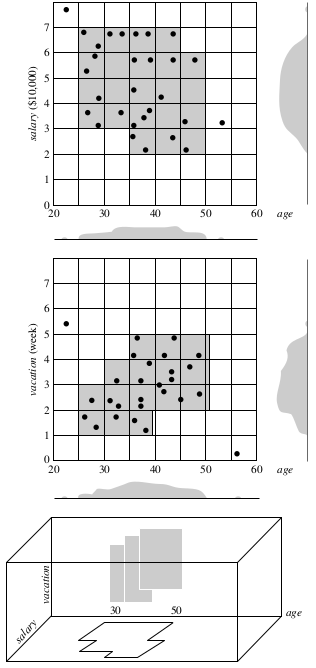
\includegraphics[height=0.6\textheight]{clique}
\caption{CLIQUE: las celdas densas encontradas con respecto a \textit{edad} (\textit{age}) para las dimensiones \textit{salario} (\textit{salary}) y \textit{vacaciones} (\textit{vacation}) se intersectan para formar un espacio de búsqeda de unidades densas de mayor dimensionalidad \cite{LIBRO}.}
\label{fig:clique}
\end{figure}

%====================================================================================================================================================%
                                              %============================================================%
%====================================================================================================================================================%


\section{Tipos de datos} \label{sec:tipos de datos}

Otro de los factores más importantes en el proceso de clusterización es conocer el tipo de dato con el que se esté trabajando, pues esto influye en gran medida a la hora de seleccionar el algoritmo de clusterización a aplicar. Muchos de los algoritmos originales de clustering fueron diseñados con la idea de tratar únicamente con datos numéricos \cite{otrolibro}, pero como se ha mencionado previamente, el imparable desarrollo de las tecnologías de la información y la comunicación ha desembocado en la generación de otro tipos de datos como imágenes, documentos, audios, videos, etc. 

Esto a su vez ha provocado el aumento de datos estructurados, semiestructurados y no estructurados. Los datos estructurados son todos aquellos que se suelen encontrar en bases de datos, donde cada campo tiene su descripción, restricciones y relaciones con otros campos y estructuras. Los datos semisupervisados provienen de información estructurada pero que no está representada con modelos de datos estructurados y bases de datos relacionales. Y por último, los datos no estructurados no guardan ningún tipo de formato ni está organizada de una forma estructurada. Estos dos últimos tipos de datos dificultan su procesamiento y hacen más costoso obtener información de ellos \cite{articulo14}.

Los diferentes categorías de datos con los que se suele trabajar de forma común dentro del mundo de la clusterización son las siguientes:

\begin{itemize}
  \item \textbf{Datos categóricos}: Se consideran datos categóricos todos aquellos que pueden ser asignadas en un número finito de categorías, tales como sexo, edad, etnia, etc. Estos son muy comunes en conjuntos de datos reales, donde además es probable que estén mezclados con otro tipo de datos numéricos.  Un ejemplo típico de este tipo de datos se da en encuestas en las que se te da a elegir entre un número limitado de opciones (\textit{p. ej.} Tipo de educación: pública o privada).
  
  Clusterizar este tipo de datos ha supuesto numerosos problemas puesto que las medidas comunes de similitud quedan obsoletas, haciendo necesario definir nuevos criterios para el cálculo de la semejanza; y por otro lado, al no tratar datos numéricos, métodos que utilizan la media o mediana deben ser modificados apropiadamente para estos datos discretos. Si a esto le sumamos que puede haber atributos mezclados en el conjuntos de datos, aumentamos la complejidad del problema.
  
  \item \textbf{Datos textuales}: Los datos de texto o documentos son un tipo de dato que siempre ha sido común, pero hasta hace pocos años predominaba en formato físico. Con el desarrollo de editores de texto, la informatización de los trabajos y el todavía creciente mundo de internet y las redes sociales estos datos abundan en su forma digital.
  
  Normalmente estos documentos se representan como un amalgama de palabras, donde cada una de ellas se considera un atributo, sin tener en cuenta el orden de aparición. Esto implica que la cantidad de atributos por cada documento es muy alta, que es el principal obstáculo que presenta la clusterización de estos datos, así como la ambiguedad de las palabras. 
  
  \item \textbf{Datos multimedia}: De la misma manera, las redes sociales e internet han favorecido la creaión de contenido multimedia que se compone de audio, imágnes y vídeos principalmente, que normalmente se encuentra acompañado de otros tipos de datos.
  
  Aplicar clusterización en este tipo de datos se ha convertido en una de las herramientas más eficaces para la obtención de información en este ámbito, pero también tiene sus complicaciones, pues en el fondo, todos ellos son tipos de datos diferentes que necesitan ser procesados de forma distinta.
  
  \item \textbf{Datos de emisiones contínuas}: Este tipo de datos, también denominados datos de ``streaming''\footnote{Este término inglés es cada vez más utilizado de forma coloquial sobre todo entre los jóvenes para referirse a retransmisiones en vivo principalemente emitidas en internet o redes sociales.} puede considerarse como un subconjunto de datos multimedia, pues estos datos suelen ser audio, vídeos o animaciones pero que se retransmiten en tiempo real. En los últimos años este tipo de datos se ha visto fuertemente incrementado gracias a plataformas como YouTube o Twitch\footnote{Plataforma que permite realizar transimisiones en vivo propiedad de Amazon, siendo una de las principales fuentes de retransimisión de videojuegos, compitiendo con YouTube} y diversas redes sociales que permiten emitir en directo a más personas.
  
  Los principales problemas que presentan este tipo de datos son el gran volumen de datos y su retransmisión en tiempo real. Esto implica que, métodos vistos en los que se necesitan varias iteraciones para clusterizar los datos no sirven, puesto que es necesario hacerlo de una sola pasada. Esto implica que la velocidad de los algoritmos debe ser elevada y con poca complejidad. Asimismo, los patrones de los datos cambian constantemente, obligando a actualizar la estructura subyacente de los mismos.
  
  \item \textbf{Series temporales}: Los datos temporales o cronológicos son obtenidos en mediciones realizadas en momentos concretos y que están ordenadas de forma secuencial, según el tiempo en el que se realizó la prueba. Algunos ejemplos sencillos son muestras de temperatura que se recogen en intervalos de tiempo constante, recuento del número de afectados por una enfermedad o incluso mediciones del control de peso de una persona.
  
  Entre los ejemplos planteados se puede diferenciar entre datos divididos en intervalos constantes o dispersos y suelen contener un tipo de valor asociado con un atributo contextual: el tiempo.
  
  La aplicación de clustering en ámbitos con este tipo de datos ayuda con la detección de entidades con tendencias similares, aunque también existen complicaciones, puesto que es dificil definir la similitud entre distintas secuencias temporales debido al hecho de que esto puede suponer grandes cambios conforme el tiempo avanza.
  
  \item \textbf{Secuencias discretas}: Cada vez más son los ámbitos que generan secuencias discretas en vez de categóricas, y que en vez de diferenciarse por el contexto temporal, lo hacen por la posición o emplazamiento. Estos datos tiene una estructura normalmente lineal y algunos ejemplos de este tipo de datos son los registros de acceso a internet o las secuencias de comandos de un ordenador. 
  
  Al contrario que datos numéricos, este tipo de datos requiere de un alto nivel computacional para su procesamiento, puesto que es complicado encontrar representantes de los datos.
  
  \item \textbf{Datos biológicos}: Los datos biológicos son el principal tipo de dato de las secuencias discretas y se centran sobretodo en datos rferentes al genoma y proteinas. Clustering se aplica en este caso con la intención de agrupar las secuencias biológicas que están relacionadas para así poder comprender mejor el funcionamiento del genoma y las tareas que realizan las células.
  
  \item \textbf{Redes y grafos}: Este tipo de datos son de los más comunes entre las represenctaciones de datos, puesto que virtualmente cada tipo de dato puede ser representado como un grafo de similitud con aristas ponderadas en función de la semejanza. 
  
  La clusterización de estos datos es una de las formas más fiables e importantes a la hora de obtener información valiosa los grafos y redes, y muchos otros problemas pueden ser afrontados si se tranforman en este tipo de datos y aplicando métodos de clusterización, sirviendo como una forma de abstracción de los datos.
  
  \item \textbf{Datos difusos}: Muchos conjuntos de datos suelen tener cierto grado de incertidumbre en los mismos, y esto puede ser medido y recolectado para mejorar los resultados de los algoritmos de Data Mining. Esto se debe al hecho de que la incertidumbre de estos datos ofrece una medida probabilística de la importancia que tiene los atributos, haciendo más efectivo su procesamiento. 
  
  Por lo tanto, es una práctica común disminuir la calidad de los datos para utilizar algoritmos que se benefician de lo mencionado previamente o simplemente utilizar herramientas de medidad imprecisas. Este puede ser el caso de sensores donde la imprecisión puede medirse de antemano o datos obtenidos de previsiones donde siempre hay cierta incertidumbre que puede ser inferida.
  
  Uno de los problemas que presentan estos datos ese que la incertidumbre se puede confundir con la de Fuzy clustering. En la clusterización relajada la incertidumbre proviene del diseño de los métodos, mientras que en los datos difusos esta es inherente a los mismos.
   
\end{itemize}

En la Tabla \ref{tab:Tabla 2} se han comparado los diferentes métodos que se han expuesto en este documento en función del tipo de dato para el que son utilizados según \cite{articulo14,otrolibro}. Como se puede ver, los métodos probabilísticos soportan todos los tipos de datos debido a su gran abstracción, pues al basarse en la estructura subyacente de los mismos, puede aplicarse de más formas. El siguiente tipo de algoritmos que más datos puede procesar son los basados en particiones, puesto que su gran sencillez permite modificarlos facilmente y adaptarlos a las necesidades pertinenetes.

\begin{table}[ht]
\renewcommand\arraystretch{2}
\centering
\resizebox{\textwidth}{!}{%
\begin{tabular}{|c|c|c|c|c|c|c|c|c|}
\hline
\textbf{\begin{tabular}[c]{@{}c@{}}Métodos\\ /Tipo de dato\end{tabular}} & \textbf{Particiones} & \textbf{Jerárquicos} & \textbf{Densidad} & \textbf{Rejilla} & \textbf{Fuzzy} & \textbf{Probabilísticos} & \textbf{Grafos} & \textbf{Redes nuronales} \\ \hline
\textbf{Categórico} & \checkmark & \checkmark & \checkmark & \checkmark & \checkmark & \checkmark &  &  \\ \hline
\textbf{Texto} & \checkmark & \checkmark & \checkmark &  & \checkmark & \checkmark & \checkmark & \checkmark \\ \hline
\textbf{Multimedia} & \checkmark & \checkmark &  &  &  & \checkmark & \checkmark &  \\ \hline
\textbf{Streaming} & \checkmark &  & \checkmark & \checkmark &  & \checkmark & \checkmark &  \\ \hline
\textbf{Temporales} & \checkmark & \checkmark & \checkmark & \checkmark &  & \checkmark &  &  \\ \hline
\textbf{Discretos} & \checkmark &  &  &  &  & \checkmark &  &  \\ \hline
\textbf{Biológicos} & \checkmark & \checkmark &  & \checkmark &  & \checkmark & \checkmark & \checkmark \\ \hline
\textbf{Red} &  & \checkmark &  &  & \checkmark & \checkmark & \checkmark & \checkmark \\ \hline
\textbf{Difusos} & \checkmark &  & \checkmark & \checkmark &  & \checkmark &  &  \\ \hline
\end{tabular}%
}
\caption{Comparativa entre los métodos de clusterización y los tipos de datos con los que suelen trabajar.}
\label{tab:Tabla 2}
\end{table}


%====================================================================================================================================================%
                                              %============================================================%
%====================================================================================================================================================%


\section{Evaluación del clustering} \label{sec:Evaluación del clustering}

Las técnicas y algoritmos que se han expuesto son tan solo los más populares, una pequeña parte de todos los que existen, pues existen múltiples variaciones, nuevas versiones y combinaciones de cada uno de ellos enfocados en mejorar el rendimiento, cubrir flaquezas y permitir nuevas aplicaciones y funcionalidades.

Sin embargo, ¿cómo sabemos que el resultado de una clusterización es preciso y correcto?  Es necesario evaluar la clasificación final de un proceso de clustering y y los pasos iniciales para cerciorarnos de que el método utilizado y los valores asignados a las variables pertinentes son los adecuados. Gracias a esto, se pueden determinar los puntos fuertes de los algoritmos e identificar aquellas condiciones, valores y tipos de datos bajo los que ofrece mejores resultados.

Para valorar el resultado de una clusterización se suelen realizar tres tareas:

\begin{itemize}
  \item \textbf{Evaluar la tendencia de la clasificación}: Intentar determinar si existe una estructura no aleatoria en la distribución de los datos antes de custerizarlos es crucial para obtener buenos resultados. Aplicar un método de clustering a un conjunto de datos aleatorio no devolverá resultados útiles y con significado, pues los clusters que se pueden formar serán también aleatorios y por lo tanto no aportarán información. Para esto, se suele usar un procedimiento similar al de los métodos jerárquicos probabilísticos \ref{subsec:Métodos jerárquicos probabilísticos} en el que se calcula la probabilidad de que el conjunto de datos con el que se quiere trabajar haya sido generado por una distribución de datos uniforme. Uno de los procedimientos más comunes es la Estadística de Hopkins. 
  
  \item \textbf{Determinar el número de clusters}: En algunos algoritmos como $k$-means \ref{subsec:k-means} el número final de clusters es solicitado al usuario y por lo tanto debe aproximarse de antemano. Sin embargo, es una buena práctica calcular este valor antes de utilizar cualquier método para contrastar el resultado final. Esta tarea aunque ciertamente complicada, pues los factores de los que depende son muchos (distribución de los datos, número de atributos, cantidad de datos...) y para la que existen numerosas formas de calcularla, puede ser simplificada para un mayor entendimiento o fácil aplicación.  Uno de los métodos más sencillos es aproximar el número de clusters a $\sqrt{\frac{n}{2}}$, donde en cada cluster debería haber $\sqrt{2 \cdotp n}$ objetos, para un conjunto de $n$ datos. Otro métodos es Elbow Method, en el que se repite de forma iterativa el proceso de clusterización variando el valor de $k$ (número de clusters) y calculando la varianza de los puntos dentro de los clusters. Una vez termina el proceso, se muestran los resultados en un gráfico y se escoge como valor para $k$ el punto de la gráfica en el que esta se curva de forma severa tal y como se puede observar en la Figura \ref{fig:elbow}, donde el valor escogido para $k$ es tres. Este proceso también es utilizado para determinar más parámetros dentro de otros algoritmos como \textit{Epsilon} pada DBSCAN. 
  
\begin{figure}[ht]
\centering
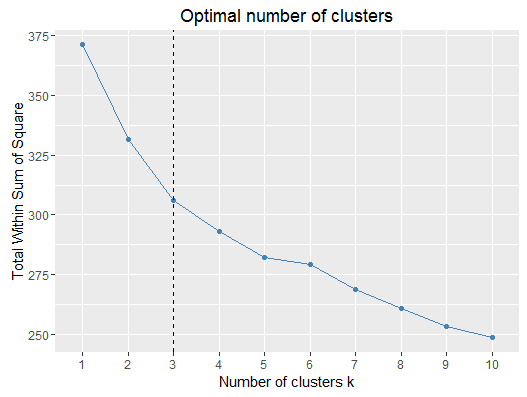
\includegraphics[width=0.6\linewidth]{elbow}
\caption{Elbow Method para encontrar el número de clusters óptimo \cite{elbow}.}
\label{fig:elbow}
\end{figure}
  
  \item \textbf{Calcular la calidad de la clusterización}: Una vez los datos han sido clasificados, se debe verificar que el resultado es bueno. Para ello se pueden usar principalmente dos aproximaciones: comprobar si los clusters acogen bien los datos (métodos intrínsecos)  o si los clusters se aproximan a una realidad existente (métodos extrínsecos), que suele ser una clasificación ideal realizada por expertos en la materia. 
  
  Los métodos extrínsecos intentan puntuar la clusterización obtenida $C$ comparándola con una realidad $C_g$ basándose en cuatro conceptos fundamentales: la homogeneidad del cluster, la integridad del cluster, la pureza del cluster y la preservación de clusters pequeños. Mientras que los métodos intrínsecos se centran en lo compactos que son los clusters y la separación entre ellos calculando la proximidad entre objetos.
\end{itemize}


%====================================================================================================================================================%
                                              %============================================================%
%====================================================================================================================================================%

\section{Aplicaciones de clustering} \label{sec:aplicaciones}

Como se ha mencionado previamente en la Sección \ref{clustering}, la clusterización ha probado ser uno de los métodos más eficaces a la hora de obtener información de los datos mediante su clasificación y etiquetado por similitud, motivo por lo que es empleado de manera recurrente en muchos de los campos más influyentes e importantes del mundo moderno tales como ingeniería, ciencias de la computación, ciencias de la salud, ciencias sociales o economía. 

Durante este documento se han nombrado algunos de los dominios de aplicación más comunes en los que clustering ha demostrado ser una técnica súmamante útil. Ahora vamos a ampliar dicha información con la encontrada en \cite{otrolibro}. Dichos dominios son los siguientes:

\begin{itemize}
  \item \textbf{Paso intermedio para otros métodos de data mining}: El proceso de clusterización sirve tanto para etiquetar y clasificar un conjunto de datos como para sumarizar la información de los mismos, haciendo que sea un paso intermedio clave para otro tipo de métodos como clasificación supervisada\footnote{Método de Data Mining que define un modelo de clasificación que permite obtener el valor desconocido de un suceso elemental a partir del resto de valores dado un conjunto de datos sobre el que conocemos todos los posibles valores que puede tomar dicho valor desconocido.} o detección de outliers.
  
  \item \textbf{Método de filtrado colaborativo}: Este tipo de filtros en los que múltiples usuarios puntúan o evalúan algo se vale de la clusterización para encontrar aquellos usuarios con respuestas similares, permitiendo utilizar esta información en gran variedad de formas, sobretodo en sistemas recomendadores.
  
  \item \textbf{Segmentación de clientes}: Esta aplicación es una variación de los métodos de filtro colaborativos específica para clientes, que se agrupan por similitud de preferencias o gustos. La principal diferencia con el anterior es que en vez de usar las evaluaciones de los usuarios, aquí se utilizan atributos arbitrarios de los consumidores \cite{13}.
  
  \item \textbf{Resumir datos}: Muchas técnicas de clusterización están relacionadas con métodos de reducción de dimensiones en los datos, es decir, eliminar los atributos que no sean relevantes. Esto permite obtener cierta forma de resumen del conjunto de datos, que es muy útil a la hora de crear representaciones compactas de los datos, haciendo que el procesamiento e interpretamiento de los mismos sea más sencillo.
  
  \item \textbf{Detección de tendencias dinámicas}: Los métodos de clusterización dinámicos y fluidos son usados para detectar la dirección de los datos y encontrar patrones de cambio en ellos.
  
  \item \textbf{Análisis de datos multimedia}: Los datos multiemedia están compuestos por imágenes, vídeos y audios. Clustering se aplica en este tipo de datos muchas veces con intención de detectar segmentos similares para la clasificación de tipos de música, detección de infracciones de derechos de autor, etc.
  
  \item \textbf{Análisis de redes sociales}: El continuo crecimiento de las redes sociales ha dado mucha importancia a este ámbito en el que clustering se utiliza para detectar estructuras sociales o comunidades subyacentes dentro de los datos. Encontrar comunidades sirve para entender mejor cómo funciona la red social y para recomendar a usuarios de una comunidad otras similares a sus gustos \cite{11}.
  
  \item \textbf{Análisis de datos biológicos}: Los datos biológicos se han convertido en datos importantes gracias al éxito de los análisis del genoma humano\footnote{El genoma es el conjunto de genes contenidos en los cromosomas.} y la capacidad de recolectar diferentes tipos de expresión génica\footnote{La expresión génica es el proceso mediante el cual todos los organismos transforman la información codificada por los ácidos nucleicos en las proteinas necesarias para su desarrollo, fincionamiento y reproducción con otros organismos.}. Este tipo de datos suelen estructurarse como secuencias o redes, y aplicando clustering podemos detectar secuaencias inusuales y su tendencia. 
\end{itemize}


Y aunque dentro de la misma Sección \ref{clustering} se han expuesto varios ejemplos de aplicaciones de clustering en dichos ámbitos, a continuación exploraremos un poco más en detalle qué aporta esta técnica en las áreas de data mining, motores de búsqueda web, educación, procesamiento de imágenes, aprendizaje automático y bioinformática, donde se han obtenido resultados muy importantes gracias a su uso \cite{articulo14}.



%====================================================================================================================================================%
                                              %============================================================%
%====================================================================================================================================================%

\begin{comment}

\clearpage

    \begin{tcolorbox}[breakable, size=fbox, boxrule=1pt, pad at break*=1mm,colback=cellbackground, colframe=cellborder]
\prompt{In}{incolor}{14}{\boxspacing}
\begin{Verbatim}[commandchars=\\\{\}]
\PY{n+nf}{if }\PY{p}{(}\PY{o}{!}\PY{n+nf}{require}\PY{p}{(}\PY{n}{cluster}\PY{p}{)}\PY{p}{)}\PY{p}{\PYZob{}}
  \PY{n+nf}{install.packages}\PY{p}{(}\PY{l+s}{\PYZdq{}}\PY{l+s}{cluster\PYZdq{}}\PY{p}{,} \PY{n}{repos}\PY{o}{=}\PY{l+s}{\PYZsq{}}\PY{l+s}{http://cran.us.r\PYZhy{}project.org\PYZsq{}}\PY{p}{)}
\PY{p}{\PYZcb{}}
\PY{n+nf}{if }\PY{p}{(}\PY{o}{!}\PY{n+nf}{require}\PY{p}{(}\PY{n}{purrr}\PY{p}{)}\PY{p}{)}\PY{p}{\PYZob{}}
  \PY{n+nf}{install.packages}\PY{p}{(}\PY{l+s}{\PYZdq{}}\PY{l+s}{purrr\PYZdq{}}\PY{p}{,} \PY{n}{repos}\PY{o}{=}\PY{l+s}{\PYZsq{}}\PY{l+s}{http://cran.us.r\PYZhy{}project.org\PYZsq{}}\PY{p}{)}
\PY{p}{\PYZcb{}}
\PY{n+nf}{if }\PY{p}{(}\PY{o}{!}\PY{n+nf}{require}\PY{p}{(}\PY{n}{fpc}\PY{p}{)}\PY{p}{)}\PY{p}{\PYZob{}}
  \PY{n+nf}{install.packages}\PY{p}{(}\PY{l+s}{\PYZdq{}}\PY{l+s}{fpc\PYZdq{}}\PY{p}{,} \PY{n}{repos}\PY{o}{=}\PY{l+s}{\PYZsq{}}\PY{l+s}{http://cran.us.r\PYZhy{}project.org\PYZsq{}}\PY{p}{)}
\PY{p}{\PYZcb{}}
\PY{n+nf}{if }\PY{p}{(}\PY{o}{!}\PY{n+nf}{require}\PY{p}{(}\PY{n}{dbscan}\PY{p}{)}\PY{p}{)}\PY{p}{\PYZob{}}
  \PY{n+nf}{install.packages}\PY{p}{(}\PY{l+s}{\PYZdq{}}\PY{l+s}{dbscan\PYZdq{}}\PY{p}{,} \PY{n}{repos}\PY{o}{=}\PY{l+s}{\PYZsq{}}\PY{l+s}{http://cran.us.r\PYZhy{}project.org\PYZsq{}}\PY{p}{)}
\PY{p}{\PYZcb{}}
\PY{n+nf}{if }\PY{p}{(}\PY{o}{!}\PY{n+nf}{require}\PY{p}{(}\PY{n}{factoextra}\PY{p}{)}\PY{p}{)}\PY{p}{\PYZob{}}
  \PY{n+nf}{install.packages}\PY{p}{(}\PY{l+s}{\PYZdq{}}\PY{l+s}{factoextra\PYZdq{}}\PY{p}{,} \PY{n}{repos}\PY{o}{=}\PY{l+s}{\PYZsq{}}\PY{l+s}{http://cran.us.r\PYZhy{}project.org\PYZsq{}}\PY{p}{)}
\PY{p}{\PYZcb{}}
\PY{n+nf}{if }\PY{p}{(}\PY{o}{!}\PY{n+nf}{require}\PY{p}{(}\PY{n}{Matrix}\PY{p}{)}\PY{p}{)}\PY{p}{\PYZob{}}
  \PY{n+nf}{install.packages}\PY{p}{(}\PY{l+s}{\PYZdq{}}\PY{l+s}{Matrix\PYZdq{}}\PY{p}{,} \PY{n}{repos}\PY{o}{=}\PY{l+s}{\PYZsq{}}\PY{l+s}{http://cran.us.r\PYZhy{}project.org\PYZsq{}}\PY{p}{)}
\PY{p}{\PYZcb{}}
\PY{n+nf}{if }\PY{p}{(}\PY{o}{!}\PY{n+nf}{require}\PY{p}{(}\PY{n}{xtable}\PY{p}{)}\PY{p}{)}\PY{p}{\PYZob{}}
  \PY{n+nf}{install.packages}\PY{p}{(}\PY{l+s}{\PYZdq{}}\PY{l+s}{xtable\PYZdq{}}\PY{p}{,} \PY{n}{repos}\PY{o}{=}\PY{l+s}{\PYZsq{}}\PY{l+s}{http://cran.us.r\PYZhy{}project.org\PYZsq{}}\PY{p}{)}
\PY{p}{\PYZcb{}}
\PY{n+nf}{library}\PY{p}{(}\PY{n}{cluster}\PY{p}{)}
\PY{n+nf}{library}\PY{p}{(}\PY{n}{purrr}\PY{p}{)}
\PY{n+nf}{library}\PY{p}{(}\PY{n}{fpc}\PY{p}{)}
\PY{n+nf}{library}\PY{p}{(}\PY{n}{dbscan}\PY{p}{)}
\PY{n+nf}{library}\PY{p}{(}\PY{n}{factoextra}\PY{p}{)}
\PY{n+nf}{library}\PY{p}{(}\PY{n}{Matrix}\PY{p}{)}
\PY{n+nf}{library}\PY{p}{(}\PY{n}{xtable}\PY{p}{)}
\end{Verbatim}
\end{tcolorbox}

    \begin{tcolorbox}[breakable, size=fbox, boxrule=1pt, pad at break*=1mm,colback=cellbackground, colframe=cellborder]
\prompt{In}{incolor}{19}{\boxspacing}
\begin{Verbatim}[commandchars=\\\{\}]
\PY{n}{pokemon} \PY{o}{\PYZlt{}\PYZhy{}} \PY{n+nf}{read.csv}\PY{p}{(}\PY{l+s}{\PYZdq{}}\PY{l+s}{Pokemon.csv\PYZdq{}}\PY{p}{,} \PY{n}{encoding}\PY{o}{=}\PY{l+s}{\PYZdq{}}\PY{l+s}{UTF\PYZhy{}8\PYZdq{}}\PY{p}{,} \PY{n}{header}\PY{o}{=}\PY{k+kc}{TRUE}\PY{p}{,} \PY{n}{sep}\PY{o}{=}\PY{l+s}{\PYZdq{}}\PY{l+s}{,\PYZdq{}}\PY{p}{,} \PY{n}{strip.white}\PY{o}{=}\PY{k+kc}{TRUE}\PY{p}{)}\PY{n}{[} \PY{p}{,}\PY{n+nf}{c}\PY{p}{(}\PY{l+s}{\PYZsq{}}\PY{l+s}{Name\PYZsq{}}\PY{p}{,} \PY{l+s}{\PYZsq{}}\PY{l+s}{Total\PYZsq{}}\PY{p}{)}\PY{n}{]}
\PY{n}{pokemon} \PY{o}{\PYZlt{}\PYZhy{}} \PY{n+nf}{data.frame}\PY{p}{(}\PY{n}{pokemon}\PY{p}{)}
\PY{n}{pokemon\PYZus{}fig} \PY{o}{\PYZlt{}\PYZhy{}} \PY{n+nf}{head}\PY{p}{(}\PY{n}{pokemon}\PY{p}{,} \PY{l+m}{10}\PY{p}{)}
\PY{n}{pokemon\PYZus{}fig}
\end{Verbatim}
\end{tcolorbox}

    A data.frame: 10 × 2
\begin{tabular}{r|ll}
  & Name & Total\\
  & <fct> & <int>\\
\hline
	1 & Bulbasaur                 & 318\\
	2 & Ivysaur                   & 405\\
	3 & Venusaur                  & 525\\
	4 & VenusaurMega Venusaur     & 625\\
	5 & Charmander                & 309\\
	6 & Charmeleon                & 405\\
	7 & Charizard                 & 534\\
	8 & CharizardMega Charizard X & 634\\
	9 & CharizardMega Charizard Y & 634\\
	10 & Squirtle                  & 314\\
\end{tabular}


    
    \begin{tcolorbox}[breakable, size=fbox, boxrule=1pt, pad at break*=1mm,colback=cellbackground, colframe=cellborder]
\prompt{In}{incolor}{22}{\boxspacing}
\begin{Verbatim}[commandchars=\\\{\}]
\PY{n}{d} \PY{o}{\PYZlt{}\PYZhy{}} \PY{n+nf}{dist}\PY{p}{(}\PY{n}{pokemon}\PY{p}{,} \PY{n}{method}\PY{o}{=}\PY{l+s}{\PYZdq{}}\PY{l+s}{euclidian\PYZdq{}}\PY{p}{)}
\PY{n}{hc1} \PY{o}{\PYZlt{}\PYZhy{}} \PY{n+nf}{hclust}\PY{p}{(}\PY{n}{d}\PY{p}{,} \PY{n}{method}\PY{o}{=}\PY{l+s}{\PYZdq{}}\PY{l+s}{complete\PYZdq{}}\PY{p}{)}
\PY{n}{hc1} \PY{o}{\PYZlt{}\PYZhy{}} \PY{n+nf}{as.dendrogram}\PY{p}{(}\PY{n}{hc1}\PY{p}{)}
\PY{n+nf}{par}\PY{p}{(}\PY{n}{mar} \PY{o}{=} \PY{n+nf}{c}\PY{p}{(}\PY{l+m}{2}\PY{p}{,}\PY{l+m}{0}\PY{p}{,}\PY{l+m}{0}\PY{p}{,}\PY{l+m}{0}\PY{p}{)}\PY{p}{)}
\PY{n}{nodePar} \PY{o}{\PYZlt{}\PYZhy{}} \PY{n+nf}{list}\PY{p}{(}\PY{n}{lab.cex}\PY{o}{=}\PY{l+m}{0.6}\PY{p}{,} \PY{n}{pch}\PY{o}{=}\PY{n+nf}{c}\PY{p}{(}\PY{k+kc}{NA}\PY{p}{,} \PY{l+m}{19}\PY{p}{)}\PY{p}{,} \PY{n}{cex}\PY{o}{=}\PY{l+m}{0.7}\PY{p}{,} \PY{n}{col}\PY{o}{=}\PY{l+s}{\PYZdq{}}\PY{l+s}{blue\PYZdq{}}\PY{p}{)}
\PY{n+nf}{plot}\PY{p}{(}\PY{n}{hc1}\PY{p}{,} \PY{n}{nodePar}\PY{o}{=}\PY{n}{nodePar}\PY{p}{,} \PY{n}{edgePar}\PY{o}{=}\PY{n+nf}{list}\PY{p}{(}\PY{n}{col}\PY{o}{=}\PY{l+m}{2}\PY{o}{:}\PY{l+m}{3}\PY{p}{,} \PY{n}{lwd}\PY{o}{=}\PY{l+m}{2}\PY{o}{:}\PY{l+m}{1}\PY{p}{)}\PY{p}{,} \PY{n}{labels}\PY{o}{=}\PY{k+kc}{NULL}\PY{p}{,} \PY{n}{cex}\PY{o}{=}\PY{l+m}{0.6}\PY{p}{,} \PY{n}{xlim}\PY{o}{=}\PY{n+nf}{c}\PY{p}{(}\PY{l+m}{0}\PY{p}{,}\PY{l+m}{35}\PY{p}{)}\PY{p}{,} \PY{n}{ylim}\PY{o}{=}\PY{n+nf}{c}\PY{p}{(}\PY{l+m}{0}\PY{p}{,}\PY{l+m}{6}\PY{p}{)}\PY{p}{)}
\end{Verbatim}
\end{tcolorbox}

    \begin{Verbatim}[commandchars=\\\{\}]
Warning message in dist(pokemon, method = "euclidian"):
"NAs introducidos por coerción"
    \end{Verbatim}

    \begin{center}
    \adjustimage{max size={0.9\linewidth}{0.9\paperheight}}{output_3_1.png}
    \end{center}
    { \hspace*{\fill} \\}
    
    \begin{tcolorbox}[breakable, size=fbox, boxrule=1pt, pad at break*=1mm,colback=cellbackground, colframe=cellborder]
\prompt{In}{incolor}{24}{\boxspacing}
\begin{Verbatim}[commandchars=\\\{\}]
\PY{n}{hc2} \PY{o}{\PYZlt{}\PYZhy{}} \PY{n+nf}{agnes}\PY{p}{(}\PY{n}{d}\PY{p}{,} \PY{n}{method}\PY{o}{=}\PY{l+s}{\PYZdq{}}\PY{l+s}{complete\PYZdq{}}\PY{p}{)}
\PY{n}{m} \PY{o}{\PYZlt{}\PYZhy{}} \PY{n+nf}{c}\PY{p}{(} \PY{l+s}{\PYZdq{}}\PY{l+s}{average\PYZdq{}}\PY{p}{,} \PY{l+s}{\PYZdq{}}\PY{l+s}{single\PYZdq{}}\PY{p}{,} \PY{l+s}{\PYZdq{}}\PY{l+s}{complete\PYZdq{}}\PY{p}{,} \PY{l+s}{\PYZdq{}}\PY{l+s}{ward\PYZdq{}}\PY{p}{)}
\PY{n+nf}{names}\PY{p}{(}\PY{n}{m}\PY{p}{)} \PY{o}{\PYZlt{}\PYZhy{}} \PY{n+nf}{c}\PY{p}{(} \PY{l+s}{\PYZdq{}}\PY{l+s}{average\PYZdq{}}\PY{p}{,} \PY{l+s}{\PYZdq{}}\PY{l+s}{single\PYZdq{}}\PY{p}{,} \PY{l+s}{\PYZdq{}}\PY{l+s}{complete\PYZdq{}}\PY{p}{,} \PY{l+s}{\PYZdq{}}\PY{l+s}{ward\PYZdq{}}\PY{p}{)}
\PY{n}{ac} \PY{o}{\PYZlt{}\PYZhy{}} \PY{n+nf}{function}\PY{p}{(}\PY{n}{x}\PY{p}{)} \PY{p}{\PYZob{}}
    \PY{n+nf}{agnes}\PY{p}{(}\PY{n}{d}\PY{p}{,}\PY{n}{method}\PY{o}{=}\PY{n}{x}\PY{p}{)}\PY{o}{\PYZdl{}}\PY{n}{ac}
\PY{p}{\PYZcb{}}
\PY{n+nf}{map\PYZus{}dbl}\PY{p}{(}\PY{n}{m}\PY{p}{,} \PY{n}{ac}\PY{p}{)}
\end{Verbatim}
\end{tcolorbox}

    \begin{description*}
\item[average] 0.999318908624144
\item[single] 0.996050000000001
\item[complete] 0.999622916666667
\item[ward] 0.999933844937563
\end{description*}


    
    \begin{tcolorbox}[breakable, size=fbox, boxrule=1pt, pad at break*=1mm,colback=cellbackground, colframe=cellborder]
\prompt{In}{incolor}{27}{\boxspacing}
\begin{Verbatim}[commandchars=\\\{\}]
\PY{n}{hc3} \PY{o}{\PYZlt{}\PYZhy{}} \PY{n+nf}{as.dendrogram}\PY{p}{(}\PY{n+nf}{agnes}\PY{p}{(}\PY{n}{d}\PY{p}{,} \PY{n}{method}\PY{o}{=}\PY{l+s}{\PYZdq{}}\PY{l+s}{ward\PYZdq{}}\PY{p}{)}\PY{p}{)}
\PY{n+nf}{par}\PY{p}{(}\PY{n}{mar} \PY{o}{=} \PY{n+nf}{c}\PY{p}{(}\PY{l+m}{2}\PY{p}{,}\PY{l+m}{0}\PY{p}{,}\PY{l+m}{0}\PY{p}{,}\PY{l+m}{0}\PY{p}{)}\PY{p}{)}
\PY{n+nf}{plot}\PY{p}{(}\PY{n}{hc3}\PY{p}{,} \PY{n}{nodePar}\PY{o}{=}\PY{n}{nodePar} \PY{p}{,}\PY{n}{edgePar}\PY{o}{=}\PY{n+nf}{list}\PY{p}{(}\PY{n}{col}\PY{o}{=}\PY{l+m}{2}\PY{o}{:}\PY{l+m}{3}\PY{p}{,} \PY{n}{lwd}\PY{o}{=}\PY{l+m}{2}\PY{o}{:}\PY{l+m}{1}\PY{p}{)}\PY{p}{,} \PY{n}{labels}\PY{o}{=}\PY{k+kc}{NULL}\PY{p}{,} \PY{n}{cex}\PY{o}{=}\PY{l+m}{0.6}\PY{p}{,} \PY{n}{xlim}\PY{o}{=}\PY{n+nf}{c}\PY{p}{(}\PY{l+m}{0}\PY{p}{,}\PY{l+m}{35}\PY{p}{)}\PY{p}{,} \PY{n}{ylim}\PY{o}{=}\PY{n+nf}{c}\PY{p}{(}\PY{l+m}{0}\PY{p}{,}\PY{l+m}{8}\PY{p}{)}\PY{p}{)}
\end{Verbatim}
\end{tcolorbox}

    \begin{center}
    \adjustimage{max size={0.9\linewidth}{0.9\paperheight}}{output_5_0.png}
    \end{center}
    { \hspace*{\fill} \\}
    
    \begin{tcolorbox}[breakable, size=fbox, boxrule=1pt, pad at break*=1mm,colback=cellbackground, colframe=cellborder]
\prompt{In}{incolor}{28}{\boxspacing}
\begin{Verbatim}[commandchars=\\\{\}]
\PY{n}{hc4} \PY{o}{\PYZlt{}\PYZhy{}} \PY{n+nf}{diana}\PY{p}{(}\PY{n}{d}\PY{p}{)}
\PY{n}{hc4d} \PY{o}{\PYZlt{}\PYZhy{}} \PY{n+nf}{as.dendrogram}\PY{p}{(}\PY{n}{hc4}\PY{p}{)}
\PY{n+nf}{par}\PY{p}{(}\PY{n}{mar} \PY{o}{=} \PY{n+nf}{c}\PY{p}{(}\PY{l+m}{2}\PY{p}{,}\PY{l+m}{0}\PY{p}{,}\PY{l+m}{0}\PY{p}{,}\PY{l+m}{0}\PY{p}{)}\PY{p}{)}
\PY{n+nf}{plot}\PY{p}{(}\PY{n}{hc4d}\PY{p}{,} \PY{n}{nodePar}\PY{o}{=}\PY{n}{nodePar} \PY{p}{,}\PY{n}{edgePar}\PY{o}{=}\PY{n+nf}{list}\PY{p}{(}\PY{n}{col}\PY{o}{=}\PY{l+m}{2}\PY{o}{:}\PY{l+m}{3}\PY{p}{,} \PY{n}{lwd}\PY{o}{=}\PY{l+m}{2}\PY{o}{:}\PY{l+m}{1}\PY{p}{)}\PY{p}{,} \PY{n}{labels}\PY{o}{=}\PY{k+kc}{NULL}\PY{p}{,} \PY{n}{cex}\PY{o}{=}\PY{l+m}{0.6}\PY{p}{,} \PY{n}{xlim}\PY{o}{=}\PY{n+nf}{c}\PY{p}{(}\PY{l+m}{0}\PY{p}{,}\PY{l+m}{30}\PY{p}{)}\PY{p}{,} \PY{n}{ylim}\PY{o}{=}\PY{n+nf}{c}\PY{p}{(}\PY{l+m}{0}\PY{p}{,}\PY{l+m}{8}\PY{p}{)}\PY{p}{)}
\end{Verbatim}
\end{tcolorbox}

    \begin{center}
    \adjustimage{max size={0.9\linewidth}{0.9\paperheight}}{output_6_0.png}
    \end{center}
    { \hspace*{\fill} \\}
    
    \begin{tcolorbox}[breakable, size=fbox, boxrule=1pt, pad at break*=1mm,colback=cellbackground, colframe=cellborder]
\prompt{In}{incolor}{32}{\boxspacing}
\begin{Verbatim}[commandchars=\\\{\}]
\PY{n}{pokemon} \PY{o}{\PYZlt{}\PYZhy{}} \PY{n+nf}{head}\PY{p}{(}\PY{n}{pokemon}\PY{p}{,} \PY{l+m}{100}\PY{p}{)}
\PY{n}{d} \PY{o}{\PYZlt{}\PYZhy{}} \PY{n+nf}{dist}\PY{p}{(}\PY{n}{pokemon}\PY{p}{,} \PY{n}{method}\PY{o}{=}\PY{l+s}{\PYZdq{}}\PY{l+s}{euclidian\PYZdq{}}\PY{p}{)}
\PY{n}{hc4} \PY{o}{\PYZlt{}\PYZhy{}} \PY{n+nf}{diana}\PY{p}{(}\PY{n}{d}\PY{p}{)}
\PY{n}{clust} \PY{o}{\PYZlt{}\PYZhy{}} \PY{n+nf}{cutree}\PY{p}{(}\PY{n}{hc4}\PY{p}{,} \PY{n}{k}\PY{o}{=}\PY{l+m}{5}\PY{p}{)}
\PY{n+nf}{fviz\PYZus{}cluster}\PY{p}{(}\PY{n+nf}{list}\PY{p}{(}\PY{n}{data} \PY{o}{=} \PY{n}{d}\PY{p}{,} \PY{n}{cluster}\PY{o}{=}\PY{n}{clust}\PY{p}{)}\PY{p}{)}
\end{Verbatim}
\end{tcolorbox}

    \begin{Verbatim}[commandchars=\\\{\}]
Warning message in dist(pokemon, method = "euclidian"):
"NAs introducidos por coerción"
    \end{Verbatim}

    \begin{center}
    \adjustimage{max size={0.9\linewidth}{0.9\paperheight}}{output_7_1.png}
    \end{center}
    { \hspace*{\fill} \\}
    
    
\end{comment}
    

%====================================================================================================================================================%
                                              %============================================================%
%====================================================================================================================================================%


\clearpage

\section{Anexo}

\renewcommand{\contentsname}{\subsection{\textbf{Índice}}}
\tableofcontents

\renewcommand{\listalgorithmcfname}{\subsection{\textbf{Algoritmos}}}
\listofalgorithms

\renewcommand{\listtablename}{\subsection{\textbf{Tablas}}}
\listoftables

\renewcommand{\listfigurename}{\subsection{\textbf{Imágenes y figuras}}}
\listoffigures

\section{Referencias}
\renewcommand{\section}[2]{}
\begin{thebibliography}{X}

\bibitem{INTRODUCCION} Alberts, D. S., \& Papp, D. S. (1997). \href{http://www.dodccrp.org/files/Alberts_Anthology_I.pdf} {The information age: An anthology on its impact and consequences}. Office of the Assistant Secretary of Defense Washington DC Command and Control Research Program (CCRP).

\bibitem{DATA NEVER SLEEP} Becoming A Data-Driven CEO | Domo. (2018). Data never sleeps 6.0 \href{https://www.domo.com/solution/data-never-sleeps-6} {https://www.domo.com/solution/data-never-sleeps-6}

\bibitem{3} Xu, Z., \& Shi, Y. (2015). \href {https://link.springer.com/content/pdf/10.1007/s40745-015-0063-7.pdf} {Exploring big data analysis: fundamental scientific problems}´. Annals of Data Science, 2(4), 363-372.

\bibitem{4} Definición Data Science apuntes FCD

\bibitem{6} The R Project for Statistical Computing. (n.d.). Retrieved from \href{https://www.r-project.org/} {https://www.r-project.org/}

\bibitem{7} Moreno, A. (1994). \href{https://upcommons.upc.edu/bitstream/handle/2099.3/36157/9788483019962.pdf?sequence=1&isAllowed=y} {Aprendizaje automático.} Llibre, Edicions UPC.

\bibitem{8} Apuntes JJ clustering

\bibitem{survey} Xu, R., \& Wunschii, D. (2005). Survey of Clustering Algorithms. IEEE Transactions on Neural Networks, 16(3), 645-678. doi:10.1109/tnn.2005.845141

\bibitem{9} Alkhaibari, A. A., \& Chung, P. (2017). \href{https://ieeexplore.ieee.org/document/8001983} {Cluster analysis for reducing city crime rates}. 2017 IEEE Long Island Systems, Applications and Technology Conference (LISAT). doi:10.1109/lisat.2017.8001983

\bibitem{10} Song, Y., Meng, H., \& Zhang, Y. (2010). \href{https://ieeexplore.ieee.org/document/5602787} {Clustering analysis and its applications}. 2010 Second IITA International Conference on Geoscience and Remote Sensing. doi:10.1109/iita-grs.2010.5602787

\bibitem{11} Prabhu, J., Sudharshan, M., Saravanan, M., \& Prasad, G. (2010). \href{https://ieeexplore.ieee.org/document/5563072} {Augmenting Rapid Clustering Method for Social Network Analysis}. 2010 International Conference on Advances in Social Networks Analysis and Mining. doi:10.1109/asonam.2010.55

\bibitem{12} Baron, J. N., Aznar, M. N., Monterubbianesi, M., \& Martínez-López, B. (2020). \href{https://search.ebscohost.com/login.aspx?direct=true&db=aph&AN=143827917&lang=es&site=ehost-live&scope=site} {Application of network analysis and cluster analysis for better prevention and control of swine diseases in Argentina}. PLoS ONE, 15(6), 1–26. https://doi.org/10.1371/journal.pone.0234489

\bibitem{13} Li, J., \& Chen, P. (2008). \href{https://ieeexplore.ieee.org/document/4810639} {The application of Cluster analysis in Library system}. 2008 IEEE International Symposium on Knowledge Acquisition and Modeling Workshop. doi:10.1109/kamw.2008.4810639

\bibitem{articulo14} Emebo, O., Aromolaran, O., Oyelade, J., Isewon, I., Oladipupo, O., Omogbadegun, Z., ... Olawole, O. (2019). Data Clustering: Algorithms and Its Applications. 2019 19th International Conference on Computational Science and Its Applications (ICCSA). doi:10.1109/iccsa.2019.000-1

\bibitem{15} Carugo, O., \& Eisenhaber, F. (2010). Data Mining Techniques for the Life Sciences. Humana Press.

\bibitem{LIBRO}Han, J., Kamber, M., \& Pei, J. (2012). Data Mining: Concepts and Techniques (3rd ed., p.~740). 225 Wyman Street, Waltham, MA 02451, USA: Morgan Kaufmann Publishers, Elsevier.

\bibitem{17} Höppner, F., Klawonn, F., Kruse, R., \& Runkler, T. (1999). Fuzzy cluster analysis: methods for classification, data analysis and image recognition. John Wiley \& Sons.

\bibitem{teoria grafos} Harary, F. (1996). Graph theory. London: Addison-Wesley.

\bibitem{foto grafo} Foggia, Pasquale \& Percannella, Gennaro \& Vento, Mario. (2014). Graph Matching and Learning in Pattern Recognition in the Last 10 Years. International Journal of Pattern Recognition and Artificial Intelligence. doi:10.1142/S0218001414500013. 

\bibitem{kmeansfoto} Benavente, P., Protopapas, P., \& Pichara, K. (2017). Automatic Survey-invariant Classification of Variable Stars. The Astrophysical Journal, 845(2), 147. doi: 10.3847/1538-4357/aa7f2d

\bibitem{fuzzymeans} Bezdek, J. C., Ehrlich, R., \& Full, W. (1984). FCM: The fuzzy c-means clustering algorithm. Computers \& Geosciences, 10(2-3), 191-203.

\bibitem{babu} Grant, R. P., \& Babu, M. M. (2004). Computational genomics: Theory and application. Wymondham: Horizon Bioscience.

\bibitem{jerarquico} Struyf, A., Hubert, M., \& Rousseeuw, P. (1997). Clustering in an object-oriented environment. Journal of Statistical Software, 1(4), 1-30.

\bibitem{18} Sano, A. V., Imanuel, T. D., Calista, M. I., Nindito, H., \& Condrobimo, A. R. (2018). The Application of AGNES Algorithm to Optimize Knowledge Base for Tourism Chatbot. 2018 International Conference on Information Management and Technology (ICIMTech). doi:10.1109/icimtech.2018.8528174

\bibitem{birchfoto} A. Periklis. (2002). Data Clustering Techniques. University of Toronto.

\bibitem{BIRCH} T. Zhang. (n.d.). BIRCH: An efficient data clustering method for very large databases. Proc. ACM SIGMOD Conf. Management of Data, 103-114.

\bibitem{BIRCH 2} Lorbeer, B., Kosareva, A., Deva, B., Softić, D., Ruppel, P., \& Küpper, A. (2018). Variations on the Clustering Algorithm BIRCH. Big Data Research, 11, 44-53. doi: 10.1016/j.bdr.2017.09.002

\bibitem{chameleon} Karypis, G., Eui-Hong Han, \& Kumar, V. (1999). Chameleon: hierarchical clustering using dynamic modeling. Computer, 32(8), 68-75. doi: 10.1109/2.781637

\bibitem{DBSCAN} Ester, M., Kriegel, H. P., Sander, J., \& Xu, X. (1996, August). A density-based algorithm for discovering clusters in large spatial databases with noise. In Kdd (Vol. 96, No. 34, pp. 226-231).

\bibitem{DBSCAN 2} Schlitter, N., Falkowski, T., \& Laessig, J. (2011). DenGraph-HO: Density-based Hierarchical Community Detection for Explorative Visual Network Analysis. Research and Development in Intelligent Systems XXVIII, 283-296. doi:10.1007\/978-1-4471-2318-7\_22

\bibitem{DENCLUE} Hinneburg, A., \& Keim, D. A. (1998). An efficient approach to clustering in large multimedia databases with noise.

\bibitem{sting} Wang, W., Yang, J., \& Muntz, R. (1997, August). STING: A statistical information grid approach to spatial data mining. In VLDB (Vol. 97, pp. 186-195).

\bibitem{sting 2} Makhabel, B. (2015). Learning data mining with R: Develop key skills and techniques with R to create and customize data mining algorithms. Birmingham, UK: Packt Publishing.

\bibitem{elbow} Xing, Wanli. (2016). Exploring the collective knowledge curation process of online health communities´. 10.13140/RG.2.2.17964.05761. 

\bibitem{otrolibro} C. C. Aggarwal \&. K. Reddy. (2014). Data Clustering: Algorithms and Applications. Taylor \& Francis Group. LLC

\end{thebibliography}    
    
%====================================================================================================================================================%
                                              %============================================================%
%====================================================================================================================================================%    
\clearpage
\includepdf[pages=2]{Recursos/portada.pdf}
    
  
\end{document}
